\documentclass[11pt,openany]{ctexbook}
\usepackage[a4paper,margin=2.4cm,headheight=16pt]{geometry}
\usepackage{amsmath,amssymb,bm,mathtools,amsthm}
\usepackage{booktabs,array,longtable,tabularx}
\usepackage{graphicx,tikz,pgfplots}
\usetikzlibrary{arrows.meta,calc}
\pgfplotsset{compat=1.18}
\usepackage{fancyhdr,enumitem,float,placeins,microtype,needspace}
\usepackage[most]{tcolorbox}
\usepackage[colorlinks,linkcolor=blue!45!black,citecolor=green!35!black,urlcolor=blue!55!black]{hyperref}
\usepackage{xurl}
\setlength{\emergencystretch}{3em}
\setlist{nosep,leftmargin=2em}
\raggedbottom
\pagestyle{fancy}
\fancyhf{}
\fancyhead[L]{\small\nouppercase{\leftmark}}
\fancyfoot[C]{\thepage}
\newcommand{\dd}{\mathop{}\!\mathrm d}
\newcommand{\R}{\mathbb R}
\newcommand{\K}{\mathcal K}
\newcommand{\norm}[1]{\left\lVert #1\right\rVert}
\DeclareMathOperator{\diag}{diag}
\DeclareMathOperator{\tr}{tr}
\DeclareMathOperator{\nnz}{nnz}
\DeclareMathOperator{\curl}{curl}
\DeclareMathOperator{\diverg}{div}
\pdfstringdefDisableCommands{\def\textsuperscript#1{#1}}
\newtcolorbox{chaptersummary}{colback=blue!3,colframe=blue!45!black,title=本章总结,fonttitle=\bfseries,arc=1mm}
\newtcolorbox{authornote}{colback=yellow!7,colframe=orange!70!black,title=潜在认知跳跃,fonttitle=\bfseries,arc=1mm}
\newtcolorbox{askai}{colback=violet!3,colframe=violet!50!black,title=你应该问 AI,fonttitle=\bfseries,arc=1mm}
\newcommand{\learninggoals}[1]{\paragraph{学习目标}#1}
\newcommand{\studyroute}[2]{\paragraph{展开与检索}#1\par\textbf{关键词：}#2}
\newcommand{\conceptbridge}[3]{\begin{authornote}\textbf{潜在疑问：}#1\par\textbf{作者补充：}#2\par\textbf{核心概念联系：}#3\end{authornote}}
\newcommand{\aiexercise}[2]{\begin{askai}\textbf{AI 展开问题：}#1\par\textbf{进一步展开：}#2\end{askai}}
\newcommand{\costnote}[1]{\paragraph{工程成本与适用边界}#1}
\newcommand{\crossref}[1]{\paragraph{知识接口}#1}
\newcommand{\coderef}[1]{\paragraph{计算案例}位于本卷 \texttt{code\_examples/}：\par{\small\raggedright\nolinkurl{#1}\par}}

\title{数值线性代数与现代高性能计算\\[0.6em]\large Numerical Linear Algebra and Modern High-Performance Computing}
\author{Harvey Tan\\[0.6em]\large 计算物理学简明教程\quad 第 0 卷}
\date{2026 年 11 月}
\hypersetup{pdfauthor={Harvey Tan}}
\begin{document}
\frontmatter
\maketitle
\chapter*{阅读路线}\addcontentsline{toc}{chapter}{阅读路线}
科学计算中的空间离散产生有限维算子，算子的结构约束求解算法，算法的数据依赖进一步约束机器上的执行方式。本卷围绕这条联系组织矩阵分解、Krylov 子空间、预条件、多重网格与性能分析。
第一卷提供物理建模和空间离散，第二卷提供场方程的几何、约束与保结构离散。本卷以这些结果为输入，讨论如何可靠而高效地求解。
\par
前三章建立矩阵、残差和误差的共同语言；第二、三部分分别研究分解与投影；第四部分将它们组合为预条件与多层求解器；第五部分用 Roofline 分析算子实现、时间推进和并行通信。首次阅读可沿第 1、2、3、4、10、12、16、19、22、24、29 章建立主线，再回到各算法的条件和变体。
\par
每章给出学习目标、概念联系、最小算例和具体的 AI 展开问题。省略的证明、实现细节和检索关键词在相应位置列出。符号默认实数域；复数问题将转置替换为共轭转置。$N$ 通常表示代数未知量个数，网格每方向点数另记为 $n$。CPU 实验采用双精度；运行记录与代码位于本卷目录。性能估算、实际计时与未执行实验分别注明。
\tableofcontents
\mainmatter
\part{从离散方程到矩阵系统}
\chapter{为什么科学计算最终变成矩阵问题？}\label{v0ch:1}
\begin{chaptersummary}
第一、二卷的空间离散给出了有限维表示与离散通量，接下来的任务是求解这些离散方程。本章从未知量、局部耦合和边界处理出发，建立矩阵与离散算子的对应关系。这一对应关系决定后续分解与迭代法的选择，也为矩阵自由实现提供统一视角。
\end{chaptersummary}
\learninggoals{由一维 Poisson 方程写出矩阵；区分质量、刚度和 Jacobian；识别装配与矩阵自由的共同算子。}
\paragraph{核心问题}连续方程中的局部微分关系，怎样成为有限个未知量之间的耦合？

\section{从导数到五个未知量}
取 $-u''=f$ 于 $(0,1)$，$u(0)=g_0,u(1)=g_1$。设 $h=1/6$，$u_i\approx u(ih)$。内部五点满足
\[
 A\bm u=\bm b,\quad
 A=h^{-2}\begin{bmatrix}
 2&-1&0&0&0\\-1&2&-1&0&0\\0&-1&2&-1&0\\
 0&0&-1&2&-1\\0&0&0&-1&2
 \end{bmatrix},\quad
 \bm b=\begin{bmatrix}f_1+g_0/h^2\\f_2\\f_3\\f_4\\f_5+g_1/h^2\end{bmatrix}.
\]
行表示离散方程，列表示自由度。邻近差分读取三个值，因此每行至多有三个非零元；边界数据及其系数一起移至右端。取 $u=x(1-x)$、$f=2$ 时，二阶差分对该二次函数精确，可据此核验矩阵、符号与边界实现。
\conceptbridge{方程已是有限维，为什么还要区分未知量的定义？}{节点值、单元平均值和基函数系数属于不同坐标。离散算子把这些坐标映射为残量；矩阵条目同时编码试验空间、测试方式和相邻单元的相互作用。改变坐标或边界消元方式，即使连续 PDE 不变，矩阵也会改变。}{连续算子 $\longrightarrow$ 自由度与测试 $\longrightarrow$ 代数耦合。}
\section{装配、块结构与非线性}
有限元近似 $u_h=\sum_j u_j\phi_j$ 给出
\[
 M_{ij}=\int\phi_i\phi_j,\qquad
 K_{ij}=\int\nabla\phi_i\cdot\nabla\phi_j,\qquad
 M\dot{\bm u}+K\bm u=\bm f.
\]
共享支撑的基函数产生耦合；局部矩阵通过局部到全局编号装配。有限体积中，同一界面的数值通量同时进入两侧残量。DG 的体积分形成单元块，面通量形成邻接块。多物理场可形成鞍点或分块系统。谱基具有全局支撑时，微分矩阵可能稠密。
对于非线性残量 $\bm F(\bm u)=0$，Newton 修正满足
\[
 J(\bm u_k)\delta\bm u=-\bm F(\bm u_k),\qquad J_{ij}=\partial F_i/\partial u_j.
\]
$J$ 是当前状态处的线性化；它与时间离散后出现的质量项、边界处理共同决定线性系统。
\section{存储矩阵还是执行算子}
带状、块稀疏、Kronecker 和规则 stencil 均可描述相同规模的不同结构。
矩阵自由实现直接计算 $\bm v\mapsto A\bm v$，例如复用单元积分或邻点差分，省去完整条目存储；预条件仍可能使用装配的近似矩阵。
\costnote{三对角乘法时间和存储均为 $O(N)$；稠密存储为 $O(N^2)$。矩阵自由减少条目与索引读取，但会重复几何、系数或积分计算。比较对象应是同一算子及精度。}
\coderef{sparse_linear_algebra/solvers.py}
\crossref{第一卷空间离散给出 $M,K,J$ 的构造；本卷第 5、23、26 章分别讨论填充、算子指纹和数据布局。}
\aiexercise{对本章五内部点问题取 $g_0=1,g_1=2,f=0$，逐行推导右端并验证线性解析解；再用线性有限元写出质量与刚度矩阵。}{将同一差分写成 CSR 和不存矩阵的函数，比较输出，指出两者在边界处的共同约定。}
\studyroute{略去一般边界弱施加与非线性收敛证明。参考 \cite{golub,saad}。}{degrees of freedom; assembly; Jacobian; matrix-free operator}

\chapter{矩阵结构与求解难度}\label{v0ch:2}
\begin{chaptersummary}
上一章确定了矩阵所表示的离散算子。本章进一步考察对称性、正定性、非正规性与敏感性，将存储结构联系到求解难度。由此，Cholesky、CG、GMRES 和预条件方法的选择有了明确依据：先确认算法成立的条件，再分析问题敏感性与实际收敛。
\end{chaptersummary}
\learninggoals{识别 SPD 与不定系统；区分特征值、奇异值、条件数和谱半径；理解非正规例子的局限。}
\paragraph{核心问题}同样稀疏的两个矩阵，为什么可能需要完全不同的求解策略？

\section{能量结构与零空间}
实矩阵 $A=A^T$ 且 $\bm x^TA\bm x>0$（$\bm x\ne0$）称 SPD；若只保证非负，则为半正定。Dirichlet Poisson 矩阵 SPD，纯 Neumann 离散通常含常数零空间，需要兼容右端和规范条件。对称不定矩阵的二次型可正可负，例如
\[
 A_s=\begin{bmatrix}2&1\\1&0\end{bmatrix}.
\]
鞍点系统 $\left[\begin{smallmatrix}K&B^T\\B&0\end{smallmatrix}\right]$ 即使 $K$ SPD，整体也通常不定。非对称性可来自上风输运、非对称边界处理或线性化。
SPD 使 $\frac12\bm x^TA\bm x-\bm b^T\bm x$ 严格凸，Cholesky 主元为正，CG 的能量最小化及分母正性成立。非对称矩阵不能直接套用这些结论。
\section{三种尺度量}
对于可逆 $A$，
\[
 \kappa_2(A)=\norm{A}_2\norm{A^{-1}}_2
 =\frac{\sigma_{\max}(A)}{\sigma_{\min}(A)},\qquad
 \rho(A)=\max_i|\lambda_i(A)|.
\]
奇异值控制 Euclidean 范数放大，特征值描述不变方向，谱半径刻画固定迭代矩阵的渐近收敛。对于 SPD 矩阵，三者进一步联系为 $\kappa_2=\lambda_{\max}/\lambda_{\min}$；一般矩阵的条件数则由奇异值之比给出。
\conceptbridge{全部特征值都等于 1，为什么还可能难求解？}{非正规矩阵的特征向量可以接近线性相关，甚至不存在完整特征基。误差传播中的矩阵多项式范数不仅由特征值大小决定，还受特征向量条件及 Jordan 结构影响。因此谱图需要与奇异值、非正规性和实际残差历史共同解释。}{特征值位置 $\longrightarrow$ 多项式作用 $\longrightarrow$ 向量范数响应。}
\section{最小反例与网格效应}
取 $A_K=\left[\begin{smallmatrix}1&K\\0&1\end{smallmatrix}\right]$。它的特征值恒为 1，但
$A_K(0,1)^T=(K,1)^T$，且 $\kappa_2(A_K)$ 随 $K$ 增大而增长。它仍可能在精确算术下两步 GMRES 收敛，说明条件数也不是迭代次数的唯一预测量。
一维 Poisson 特征值为
\[
 \lambda_j=4h^{-2}\sin^2\frac{j\pi}{2(N+1)},\quad 1\le j\le N,
\]
因此网格细化时 $\kappa_2=O(h^{-2})$。离散更准确与代数系统更难求解可同时发生。
\costnote{完整奇异值分解对大型稀疏矩阵代价高。实际先使用 PDE 结构、边界和离散能量判断，再用小规模谱估计、残差和网格序列实验。}
\aiexercise{分别计算 $A_K$ 在 $K=1,10,100$ 时的奇异值和条件数；构造右端使 GMRES 一步和两步的残差不同。}{推导 Poisson 特征值并验证网格加倍时条件数的变化，说明该变化为何不等于所有右端的实际迭代增长。}
\crossref{本章条件用于第 6、13、15 章；第 16 章讨论预条件后的结构。}
\studyroute{略去伪谱和一般非正规收敛界。参考 \cite{trefethen,saad}。}{SPD; singular values; condition number; nonnormality; pseudospectrum}

\chapter{残差、误差与数值收敛}\label{v0ch:3}
\begin{chaptersummary}
矩阵性质明确后，还需要判断计算何时可以停止。本章通过残差与误差的精确关系连接问题敏感性、浮点实现和迭代监测，为后续算法提供统一的验收标准。核心是同时报告归一化方式与真实残差，并把线性代数误差放回离散误差和物理观测量的尺度中。
\end{chaptersummary}
\learninggoals{区分前向、后向误差和残差；设置含绝对容差的准则；识别递推残差与真实残差漂移。}
\paragraph{核心问题}软件报告收敛时，我们究竟知道了什么？

\section{可计算量与未知误差}
定义 $\bm e_k=\bm x_*-\bm x_k$，$\bm r_k=\bm b-A\bm x_k$，则
\[
 A\bm e_k=\bm r_k,\quad
 \frac{\norm{\bm e_k}}{\norm{\bm x_*}}
 \le \kappa(A)\frac{\norm{\bm r_k}}{\norm{\bm b}}\quad(\bm b\ne0).
\]
因此残差小只说明方程被近似满足；误差还受逆算子的放大影响。对 $A=\diag(1,10^{-8})$、$\bm x_*=(1,1)^T$、$\bm x_k=(1,0)^T$，相对残差约 $10^{-8}$，相对解误差却约 $1/\sqrt2$。
范数型相对后向误差可用
\[
 \eta_k=\frac{\norm{\bm b-A\bm x_k}}
 {\norm{A}\norm{\bm x_k}+\norm{\bm b}}
\]
度量：它允许 $A$ 和 $\bm b$ 在同一相对尺度内扰动，使 $\bm x_k$ 成为扰动问题的精确解。分量后向误差则使用 $|A||\bm x_k|+|\bm b|$ 逐分量归一化。
\conceptbridge{为什么不直接把残差压到机器精度？}{离散模型、输入数据和浮点运算各自限定了可辨别尺度。过度求解消耗时间而不改善目标误差；过早停止又可能污染物理量。应先分配误差预算，再用条件数、稳定性估计或目标量测试判断代数误差是否足够小。}{离散误差预算 $\longrightarrow$ 代数容差 $\longrightarrow$ 可验证结果。}
\section{停止与有限精度}
常用真实残差准则为
\[
 \norm{\bm r_k}\le
 \max(\texttt{atol},\texttt{rtol}\norm{\bm b}).
\]
$\bm b=0$ 时采用绝对阈值或初始残差尺度；$A\bm x=0$ 仍需考虑零空间。变量单位差异大时先明确行列缩放，避免某个分量主导范数。
浮点模型 $\mathrm{fl}(a\circ b)=(a\circ b)(1+\delta)$、$|\delta|\lesssim u$ 适用于正常范围内单次基本运算；消去、上溢和下溢会限制相对精度。算法稳定性描述实现对扰动的控制，条件数描述问题本身的敏感性。
Krylov 递推残差可能随舍入误差逐渐偏离 $\bm b-A\bm x_k$，因此最终验收采用重新计算的真实残差。分母过小、正交性丢失和预条件失效分别进入 breakdown 与停滞诊断，并据此决定继续迭代或切换策略。
\section{实验与监测}
对上述对角例子同时打印相对残差、相对误差和 $\eta_k$；对 Poisson 网格序列固定物理误差目标，改变 \texttt{rtol}，观察过度求解的成本。非线性 Newton 外迭代还需记录非线性残量，内层线性收敛不等于整体收敛。
\costnote{一次真实残差需要一次算子作用和范数；分布式范数通常包含全局归约。应平衡监测频率与可靠性，最终验收不省略。}
\coderef{sparse_linear_algebra/solvers.py}
\aiexercise{逐项计算本章对角例子的前向误差、相对残差与后向误差，并解释它们为何不矛盾。}{设计包含零右端、变量缩放和最大迭代数的停止逻辑；比较递推残差与重新计算残差的成本。}
\studyroute{略去分量扰动理论与残差替换的误差分析。参考 \cite{golub,templates}。}{forward error; backward error; true residual; residual replacement; inexact Newton}

\part{矩阵分解方法}
\chapter{Gaussian 消元与 LU 分解}\label{v0ch:4}
\begin{chaptersummary}
前面已经知道矩阵如何产生以及如何验收近似解。本章从消元建立第一条求解路线：将原系统转为两个三角系统。主元选择处理数值稳定性，分解与回代的分离则解释多右端项的优势。后续稀疏分解和不完全分解都沿用这个机制，只改变存储结构与精确程度。
\end{chaptersummary}
\learninggoals{手算带主元 LU；执行前后代；区分分解、求解和主元增长的成本。}
\paragraph{核心问题}消元为什么能被复用为一个求解算子？

\section{消元、置换与三角系统}
第 $k$ 步以 $a_{kk}$ 为主元，用乘子 $\ell_{ik}=a_{ik}/a_{kk}$ 更新
$a_{ij}\leftarrow a_{ij}-\ell_{ik}a_{kj}$。各步乘子组成单位下三角 $L$，剩余上三角组成 $U$。行置换累计为 $P$，得到 $PA=LU$。
求解依次进行
\[
 y_i=(P\bm b)_i-\sum_{j<i}\ell_{ij}y_j,\qquad
 x_i=\frac{y_i-\sum_{j>i}u_{ij}x_j}{u_{ii}}.
\]
部分主元每列选择剩余行中绝对值最大条目；完全主元同时搜索剩余行列，需额外列置换 $PAQ=LU$，最后恢复未知量顺序。部分主元通常有效，但最坏情形仍可能有较大元素增长。
\section{完整四阶算例}
取
\[
 A=\begin{bmatrix}0&2&1&0\\4&4&0&1\\2&0&3&1\\0&1&1&2\end{bmatrix},
 \quad \bm b=(3,9,6,4)^T.
\]
先交换前两行；第一列的非零乘子为 $\ell_{31}=1/2$。第二列主元为 2，取 $\ell_{32}=-1,\ell_{42}=1/2$；第三列取 $\ell_{43}=1/8$。于是
\[
 L=\begin{bmatrix}1&0&0&0\\0&1&0&0\\1/2&-1&1&0\\0&1/2&1/8&1\end{bmatrix},
 \quad U=\begin{bmatrix}4&4&0&1\\0&2&1&0\\0&0&4&1/2\\0&0&0&31/16\end{bmatrix}.
\]
逐项相乘验证 $LU=PA$。前代得到
$\bm y=(9,3,9/2,31/16)^T$，回代得到 $\bm x=(1,1,1,1)^T$。置换行列式为 $-1$，故 $\det A=-62$。
\conceptbridge{原矩阵可逆，首个主元为什么仍为零？}{可逆性保证存在完整求解，不保证当前行列顺序下每个消元主元非零。行交换重新选择消元坐标；浮点运算中还要避免用很小的主元放大乘子和舍入误差。}{可逆系统 $\longrightarrow$ 合适的消元顺序 $\longrightarrow$ 可稳定执行的三角分解。}
\section{成本、复用与验证}
稠密 LU 分解约 $2N^3/3$ FLOPs，两个三角求解合计约 $2N^2$ FLOPs，原位因子存储 $O(N^2)$。$s$ 个右端的总成本约为分解一次加 $s$ 次回代。块 LU 将大部分更新组织为矩阵乘法；它与逐元素消元数学等价，却具有不同缓存复用。
\costnote{分解因子可用于多右端和迭代改进；矩阵变化通常需要重新分解。报告分解后真实残差，必要时在更高精度计算残差并解修正方程。}
\coderef{sparse_linear_algebra/solvers.py}
\aiexercise{按本章顺序手算四阶矩阵的各步剩余子块、前代和回代，再用库分解交叉核验 $PA=LU$。}{将首个非零主元改为很小的数，比较无主元和部分主元的乘子、元素增长与后向误差。}
\studyroute{略去主元增长因子的最坏界与块算法的浮点误差证明。参考 \cite{golub}。}{partial pivoting; complete pivoting; growth factor; blocked LU; iterative refinement}

\chapter{稀疏 LU 与大型稀疏系统}\label{v0ch:5}
\begin{chaptersummary}
稀疏性减少了原矩阵的存储，消元却会在因子中引入新的耦合。本章用消元图解释填充，并区分排序、符号分析和数值分解。理解这些中间结构，才能估计稀疏直接法的内存与工作量，也能看出后续不完全分解为何需要截断填充。
\end{chaptersummary}
\learninggoals{识别 Schur 补填充；解释消元图与排序；给出规则二维和三维问题的条件化成本。}
\paragraph{核心问题}原矩阵很稀疏，因子为什么仍可能超出内存？

\section{消元创造邻居之间的联系}
将一个主元与其余未知量分块：
\[
 A=\begin{bmatrix}a&\bm r^T\\\bm c&B\end{bmatrix}
 \quad\Rightarrow\quad
 S=B-\bm c a^{-1}\bm r^T.
\]
即使 $B_{ij}=0$，只要 $c_i r_j\ne0$，$S_{ij}$ 就可能非零。对称图中消去一个节点会把其剩余邻居连为团。四节点星形图若先消中心，三个叶节点之间产生填充；先消叶节点可避免这一步的额外边。
\conceptbridge{为什么编号会影响内存，却不改变方程的物理解？}{对未知量重新编号只是置换坐标，但消元按编号依次形成 Schur 补。每一步保留哪些节点，决定哪些相互作用被压缩成新耦合。排序优化的是计算路径和中间结构。}{同一耦合图 $\longrightarrow$ 不同消元路径 $\longrightarrow$ 不同因子填充。}
\section{排序与两阶段分析}
最小度类排序倾向先消低连接节点；嵌套剖分通过小分隔集将图分为较独立区域，先处理内部再处理分隔集。符号分析预测非零结构、消元树和存储；数值阶段计算因子。非对称 LU 的动态主元交换可能改变预测，因此实际内存还受稳定性策略影响。
对规则、局部耦合的 $N$ 未知量椭圆问题，采用合适嵌套剖分且忽略额外主元增长时，典型估算为
\[
\begin{array}{c|cc}
 &\text{分解工作量}&\text{因子存储}\\\hline
2D&O(N^{3/2})&O(N\log N)\\
3D&O(N^2)&O(N^{4/3})
\end{array}
\]
上述估算以规则网格和指定排序为前提。二维每方向 $n$ 点时 $N\sim n^2$，三维则 $N\sim n^3$；统一未知量定义后，才能比较两种维数下的成本。
\section{Poisson 实验}
对五点 Poisson 生成 CSR，再转换为求解器使用的 CSC。分别采用自然编号与库提供的近似最小度类排序，记录 $\nnz(A)$、$\nnz(L)+\nnz(U)$、分解和回代时间。三维七点问题从较小网格开始，并随因子存储量逐步扩大规模。
\costnote{稀疏直接法常适合中等规模、较难预条件的系统和多右端问题；大型三维问题的填充与通信可能成为限制。数值重复分解、符号结构复用和多个右端的摊销应分别统计。}
\coderef{sparse_linear_algebra/solvers.py}
\aiexercise{对四节点星形 SPD 矩阵，分别先消中心与先消叶节点，写出每次 Schur 补并画填充边。}{对二维 Poisson 比较自然编号与 COLAMD 的因子非零数；说明它为何只是排序实例而非上述渐近界的证明。}
\studyroute{略去分隔定理、超节点和多波前实现。参考 \cite{golub,saad}。}{fill-in; elimination graph; nested dissection; symbolic factorization; multifrontal}

\chapter{Cholesky 与 LDL\textsuperscript{T} 分解}\label{v0ch:6}
\begin{chaptersummary}
上一章表明精确分解的成本由结构决定。对称性与正定性还能进一步减少工作和存储，本章因此引入 Cholesky；当正定性失效时，转向允许块主元的 LDL\textsuperscript{T}。区分这两种情形，为后面的 CG、MINRES 和不完全 Cholesky 建立共同条件。
\end{chaptersummary}
\learninggoals{推导 Cholesky 递推；识别不定系统的块主元；区分无主元与带置换分解。}
\paragraph{核心问题}对称性可以复用哪些计算，而正定性又额外保证什么？

\section{Cholesky 的递推与算例}
对实 SPD 矩阵，存在对角为正的下三角 $L$ 使 $A=LL^T$。
由条目等式得到
\[
 \ell_{jj}=\sqrt{a_{jj}-\sum_{k<j}\ell_{jk}^2},\qquad
 \ell_{ij}=\frac{a_{ij}-\sum_{k<j}\ell_{ik}\ell_{jk}}{\ell_{jj}}.
\]
SPD 保证每步 Schur 补仍正定，因此根号内为正。取
$A=\left[\begin{smallmatrix}4&2\\2&3\end{smallmatrix}\right]$，有
$L=\left[\begin{smallmatrix}2&0\\1&\sqrt2\end{smallmatrix}\right]$。
求解用 $L\bm y=\bm b$、$L^T\bm x=\bm y$。稠密工作约 $N^3/3$ FLOPs，只需存一半三角；稀疏时仍需排序与填充分析。
\section{不定问题与块对角主元}
一般实对称不定系统采用
\[
 PAP^T=LDL^T,
\]
其中 $L$ 单位下三角，$D$ 由 $1\times1$ 和 $2\times2$ 块组成。矩阵
$\left[\begin{smallmatrix}0&1\\1&0\end{smallmatrix}\right]$ 可逆，却无法以非零首个标量主元执行无交换 LDL\textsuperscript{T}；直接把整个矩阵作为一个二阶块即可。稳定实现需要对称主元策略。
\conceptbridge{把 Cholesky 的平方根改成带符号数，为什么还不够？}{不定性不仅意味着负主元，还允许非零耦合与零对角共存。标量主元可能不存在或过小，因此要同时交换行列并允许二阶块。鞍点系统的约束变量正是常见来源。}{正能量消元 $\longrightarrow$ 不定耦合 $\longrightarrow$ 对称块主元。}
\section{物理零空间与求解策略}
半正定矩阵若含刚体模态、常数模态或规范自由度，应先施加约束或在兼容子空间求解；直接补极小对角项会改变问题，需说明其数学作用。鞍点系统的块消元还会出现 Schur 补，可用作第 18、21 章的预条件接口。
\costnote{Cholesky 用于 SPD 系统；对称不定分解则通过主元交换维持数值稳定，并可能引入额外填充。结构检查应落实到实际离散通量、边界处理和预条件作用。}
\aiexercise{对本章 SPD 二阶矩阵完成 Cholesky 并解右端 $(1,1)^T$；对零对角可逆矩阵说明标量 LDL\textsuperscript{T} 的失败位置。}{构造带常数零空间的 Neumann Poisson 矩阵，检查右端兼容条件，再分别固定一个自由度与加入零均值约束。}
\studyroute{略去 Bunch--Kaufman 主元选择及稀疏超节点细节。参考 \cite{golub}。}{Cholesky; symmetric indefinite; block LDLT; saddle point; nullspace}

\chapter{QR 与最小二乘问题}\label{v0ch:7}
\begin{chaptersummary}
精确方程可能被观测数据、过定约束或投影问题替代，此时目标变为最小化残差。本章用正交分解处理最小二乘，说明正规方程为什么可能损失精度。QR 随后在 Arnoldi 和 GMRES 中再次出现：大型系统的投影最终转化为一个小型最小二乘问题。
\end{chaptersummary}
\learninggoals{建立最小二乘投影；比较正规方程与 QR；识别秩亏及正交化误差。}
\paragraph{核心问题}残差不能为零时，怎样选择最有意义的近似解？

\section{投影与条件数}
对于 $A\in\R^{m\times n}$、$m\ge n$，求 $\min_{\bm x}\norm{A\bm x-\bm b}_2$。满列秩时正规方程
$A^TA\bm x=A^T\bm b$ 唯一可解，但
\[
 \kappa_2(A^TA)=\kappa_2(A)^2.
\]
薄 QR 给出 $A=Q_1R$、$Q_1^TQ_1=I$，从而
\[
 R\bm x=Q_1^T\bm b,\qquad
 \bm r=(I-Q_1Q_1^T)\bm b.
\]
正交变换保持二范数，无需显式形成 $A^TA$。
\section{三种正交化机制}
MGS 将当前向量逐个减去已获得方向上的投影；它比经典一次性 Gram--Schmidt 更能抵抗某些消去误差，但病态基仍可能需要重正交化。Householder 反射 $H=I-2\bm v\bm v^T/(\bm v^T\bm v)$ 一次消去一列下方元素，适合稳定的稠密 QR。Givens 旋转只改变两个分量，适合增量消去 Hessenberg 矩阵的新条目。
\conceptbridge{为什么不把正规方程当作更小的对称系统直接求解？}{缩小尺寸的同时，正规方程把奇异值平方。若小奇异值已接近舍入误差尺度，形成乘积会削弱可辨识信息。QR 用保范数的变换保留原问题尺度；秩亏时还需秩判定和解的选择。}{最小残差 $\longrightarrow$ 正交投影 $\longrightarrow$ 稳定的小型三角问题。}
\section{最小算例与秩亏}
用三点 $(t_i,b_i)=(0,1),(1,2),(2,2)$ 拟合 $c_0+c_1t$：
\[
 A=\begin{bmatrix}1&0\\1&1\\1&2\end{bmatrix},\quad
 \bm c=(7/6,1/2)^T,\quad
 \bm r=\bm b-A\bm c=(-1/6,1/3,-1/6)^T.
\]
验证 $A^T\bm r=0$。若两列相同，最小二乘解便不唯一；列主元 QR 可辅助数值秩判定，SVD 则给出指定阈值下的最小范数解。可靠秩判定还需考察列相关性，无主元 $R$ 的小对角元可作为进一步检查的线索。
\costnote{稠密薄 QR 约 $2mn^2-2n^3/3$ FLOPs。存储 Householder 向量而非完整 $Q$ 可减少成本。稀疏 QR 仍可能填充；条件较好且性能优先时正规方程也可有明确使用范围。}
\aiexercise{对三点拟合显式构造薄 QR，验证正交残差并比较正规方程结果。}{令第二列为第一列加 $10^{-k}$ 倍独立向量，比较 QR、正规方程及 SVD 的残差和系数误差。}
\studyroute{略去后向稳定性证明、秩揭示 QR 与 SVD 算法。参考 \cite{golub,trefethen}。}{Householder QR; modified Gram Schmidt; Givens; rank revealing QR; least squares}

\chapter{不完全分解}\label{v0ch:8}
\begin{chaptersummary}
精确稀疏分解可能产生昂贵的填充，因此求解目标转向构造低成本的近似逆作用。本章介绍不完全分解如何选择和丢弃条目，并分析主元与三角求解带来的约束。它为第四部分的预条件设计建立基础：近似的价值由外层迭代改善与构造、应用成本共同衡量。
\end{chaptersummary}
\learninggoals{区分 ILU0、ILUk、ILUT 与 IC；解释丢弃和填充；把因子作为解三角系统的操作。}
\paragraph{核心问题}哪些消元信息值得保留，才能用有限内存改善迭代？

\section{截断消元}
精确 LU 的更新可能在原零位置产生条目。ILU(0) 只保留预定的原始非零模式；ILU($k$) 根据符号消元的填充层级保留条目，原始条目层级为零，经主元 $j$ 产生的新条目层级取相关路径层级之和加一，并保留最小层级。ILUT 主要用数值阈值和每行条目限制控制保留量。不同库的阈值缩放、排序和主元选项需查其定义。
获得近似 $A\approx LU=M$ 后，预条件作用是
\[
 \bm z=M^{-1}\bm r:\qquad L\bm y=\bm r,\quad U\bm z=\bm y.
\]
通常不形成显式逆矩阵。
\section{最小可视算例}
三对角 Poisson 无主元 LU 不产生带外填充，因此该例中 ILU(0) 可等于精确 LU。四节点环状图或二维五点矩阵则会出现额外填充，ILU(0) 将其中一部分丢弃，得到真正的近似分解。先比较这两个例子，才能观察丢弃机制。
IC 在对称模式下近似 $A\approx LL^T$，用于 SPD 矩阵 $A$。丢弃条目会改变消元中的 Schur 补，因此还需检查 IC 主元的正性；遇到非正主元时，可调整排序、加入位移或采用改进策略。
\conceptbridge{近似分解既然不精确，为什么还值得计算？}{外层迭代只需利用一个便宜的修正方向变换，不要求预条件器独立完成求解。保留主要局部耦合可降低外层迭代成本；代价是每次应用要执行有依赖关系的三角求解。}{精确消元成本 $\longrightarrow$ 受控截断 $\longrightarrow$ 外层迭代中的近似逆。}
\costnote{更小丢弃阈值常增大填充、构造和三角求解成本，却不保证总时间单调改善。通用 ILU 通常不对称，不能直接作为标准 PCG 的 SPD 预条件器。零主元、极小主元和并行依赖是独立风险。}
\coderef{sparse_linear_algebra/solvers.py}
\aiexercise{分别对三对角与二维五点 Poisson 执行 ILU(0)，列出被丢弃的条目并比较预条件后的真实残差。}{扫描 ILUT 丢弃阈值，记录构造时间、因子非零数、GMRES 次数及总时间，寻找成本折中。}
\studyroute{略去修改不完全分解及其谱等价证明。参考 \cite{saad,templates}。}{ILU(0); level of fill; ILUT; incomplete Cholesky; drop tolerance}

\chapter{LU-SGS 与近似分解}\label{v0ch:9}
\begin{chaptersummary}
不完全分解通过截断控制成本，LU-SGS 则从前后扫掠构造近似因子。本章将这一形式联系到对称 Gauss--Seidel，并比较固定迭代、预条件和伪时间更新三种用途。同一个扫掠算子在不同外层机制中承担不同任务，其收敛条件也随之明确。
\end{chaptersummary}
\learninggoals{展开 SGS 近似因子；实现前后扫掠；识别 CFD 对角近似与线性代数条件。}
\paragraph{核心问题}两次局部扫掠为何能够近似隐式全局耦合？

\section{近似因子与两次三角求解}
约定 $A=D+L+U$，$L,U$ 含实际条目的符号。假设 $D$ 可逆，定义
\[
 M=(D+L)D^{-1}(D+U)
   =A+LD^{-1}U.
\]
解 $M\delta\bm x=\bm r$ 等价于
\[
 (D+L)\bm y=\bm r,\qquad
 (D+U)\delta\bm x=D\bm y.
\]
于是无需形成乘积 $M$。若 $A$ 对称且 $D$ 正定，则 $U=L^T$，$M$ 为 SPD；用于标准 PCG 还要求整个预条件应用固定且对称。
\section{迭代、预条件与伪时间}
固定迭代 $\bm x_{k+1}=\bm x_k+M^{-1}(\bm b-A\bm x_k)$ 的误差矩阵为 $I-M^{-1}A$，谱半径小于 1 时收敛。作为预条件器时，同一个逆作用由外层 Krylov 方法组合，修正系数通过投影确定。
CFD 中 LU-SGS 常对 $\Delta t^{-1}M_t+J$ 使用近似对角块及近似 Jacobian 分裂；伪时间用于逼近稳态残量为零，伪步长不是实际物理时间分辨率。不同实现的对角项和边界处理必须明确。
\conceptbridge{名称中含 LU，为什么它通常不是原系统的精确 LU？}{这里先选择容易扫掠的三角部分，再用乘积近似整个算子；展开后多出的交叉项说明近似发生在哪里。精确 LU 则通过消元计算因子，使乘积严格等于置换后的矩阵。}{隐式耦合 $\longrightarrow$ 可扫掠近似 $\longrightarrow$ 误差由外层机制修正。}
\section{三点验证}
对 $A=\operatorname{tridiag}(-1,2,-1)$ 的三阶问题，显式计算 $LD^{-1}U$，再比较一次 $M^{-1}\bm r$ 与 $A^{-1}\bm r$。顺序扫掠利用已更新的相邻值；多色或块 Jacobi 并行化会改变算子，需重新检查效果。
\costnote{每次作用约为两次稀疏三角求解，存储近似 $O(\nnz A)$。串行依赖限制并行吞吐，局部块或分域可提高并行度但通常削弱全局耦合处理。}
\aiexercise{对三阶 Poisson 手算 $M$、$M^{-1}\bm r$ 和误差迭代矩阵，区分一次预条件作用与固定迭代的收敛。}{将扫掠改为红黑两色或分块版本，判断何处改变了矩阵分裂，并比较外层 GMRES 次数。}
\crossref{第 17 章给出平稳迭代统一形式，第 18 章讨论分域并行。}
\studyroute{略去具体可压缩流 Jacobian 分裂与伪时间参数估计。参考 \cite{saad}。}{LU-SGS; symmetric Gauss Seidel; approximate factorization; pseudo time stepping}

\part{Krylov 子空间方法}
\chapter{Krylov 子空间的基本思想}\label{v0ch:10}
\begin{chaptersummary}
精确与近似分解都需要访问因子，大规模问题有时更容易执行矩阵向量乘。本章因此从残差修正构造 Krylov 子空间，把求解转化为逐步增长的投影问题。后续 Arnoldi、GMRES 和 CG 共享这个空间，但选择基底与投影条件不同。核心是通过算子作用表达越来越丰富的误差修正。
\end{chaptersummary}
\learninggoals{从残差导出子空间；写出残差多项式；区分 Galerkin 与最小残差。}
\paragraph{核心问题}只会计算 $A\bm v$，如何逐步逼近 $A^{-1}\bm b$？

\section{由可执行操作生成搜索空间}
从 $\bm r_0=\bm b-A\bm x_0$ 出发，寻找
\[
 \bm x_m\in\bm x_0+\K_m(A,\bm r_0),\qquad
 \K_m=\operatorname{span}\{\bm r_0,A\bm r_0,\ldots,A^{m-1}\bm r_0\}.
\]
若 $\bm x_m-\bm x_0=q_{m-1}(A)\bm r_0$，则
\[
 \bm r_m=p_m(A)\bm r_0,\quad
 p_m(z)=1-zq_{m-1}(z),\quad p_m(0)=1.
\]
算法选择多项式，使相关误差或残差变小；无需显式形成高次幂。
\conceptbridge{如何由算子 $A$ 的反复作用构造逆作用近似？}{子空间保留 $A^k\bm r_0$ 等方向，再由投影共同确定系数。在有限维可逆系统中，关于初始残差的最小多项式具有非零常数项，因此逆作用可表示为有限阶多项式。有限精度、重启和预条件决定这一表示的实际逼近过程。}{易执行的矩阵作用 $\longrightarrow$ 多项式修正空间 $\longrightarrow$ 投影选择系数。}
\section{投影条件与最小多项式}
设试探基 $V_m$、测试基 $W_m$，要求
\[
 W_m^T(\bm r_0-AV_m\bm y)=0,\qquad
 W_m^TAV_m\bm y=W_m^T\bm r_0.
\]
Galerkin 取测试空间等于搜索空间；最小二范数残差要求残差正交于 $A\K_m$。两者并不相同。
若最小次数 $\nu$ 满足 $\mu_\nu(A)\bm r_0=0$，则精确算术中适当非重启方法至多 $\nu\le N$ 步得到解；实际使用的目标是远少于 $N$ 步。
\section{二阶手算}
取 $A=\diag(1,2)$、$\bm b=(1,1)^T$、$\bm x_0=0$。第一空间只有 $\alpha\bm b$，最小残差系数为 $\alpha=3/5$；第二空间由 $(1,1)^T,(1,2)^T$ 张成整个 $\R^2$，包含精确解 $(1,1/2)^T$。取 $\bm b=(1,0)^T$ 时一维已足够，说明初始残差参与决定有效难度。
\costnote{每步至少一次算子作用；基的存储与正交化依方法不同。矩阵自由与分布式算子可以直接作为接口，预条件通常比原始谱细节更能决定工程可行性。}
\aiexercise{对二阶例子分别用 Galerkin 和最小残差条件计算第一步，并解释两个系数为何不同。}{从 $\mu(z)=(z-1)(z-2)$ 写出该矩阵的逆多项式，说明初始残差只含一个特征方向时如何降阶。}
\studyroute{略去一般投影的稳定性界与非正规多项式逼近。参考 \cite{saad,trefethen}。}{Krylov subspace; residual polynomial; minimal polynomial; Galerkin projection}

\chapter{Arnoldi 与 Hessenberg 分解}\label{v0ch:11}
\begin{chaptersummary}
Krylov 幂向量生成了搜索空间，但逐步增强的线性相关性会影响数值计算。本章用 Arnoldi 在生成方向的同时正交化，将大型算子作用写成稳定坐标下的小型 Hessenberg 表示。下一章据此求解最小残差问题；本章的重点是建立并核验这条大、小系统之间的联系。
\end{chaptersummary}
\learninggoals{执行 MGS Arnoldi；手算前两步；解释正交丢失与 happy breakdown。}
\paragraph{核心问题}如何在不保存高次矩阵幂的条件下构造可靠子空间基？

\section{Arnoldi 递推}
令 $\beta=\norm{\bm r_0}_2$、$\bm v_1=\bm r_0/\beta$。第 $j$ 步：
\[
 \bm w=A\bm v_j;\quad
 h_{ij}=\bm v_i^T\bm w,\quad
 \bm w\leftarrow\bm w-h_{ij}\bm v_i\quad(i=1,\ldots,j);
 \qquad h_{j+1,j}=\norm{\bm w}_2.
\]
若 $h_{j+1,j}\ne0$，令 $\bm v_{j+1}=\bm w/h_{j+1,j}$。因此
\[
 AV_m=V_{m+1}\bar H_m,\qquad V_{m+1}^TV_{m+1}=I
\]
在精确算术成立，$\bar H_m$ 是 $(m+1)\times m$ 上 Hessenberg 矩阵。
\section{四阶矩阵前两步}
使用第 4 章的 $A$，取 $\bm r_0=\bm e_1$。第一步
\[
 A\bm e_1=(0,4,2,0)^T,\quad h_{11}=0,\quad
 h_{21}=2\sqrt5,\quad
 \bm v_2=(0,2,1,0)^T/\sqrt5.
\]
第二步 $A\bm v_2=(5,8,3,3)^T/\sqrt5$。依次投影得
\[
 h_{12}=\sqrt5,\quad h_{22}=19/5,\quad
 h_{32}=7/5,\quad
 \bm v_3=(0,2,-4,15)^T/(7\sqrt5),
\]
\[
 \bar H_2=\begin{bmatrix}0&\sqrt5\\2\sqrt5&19/5\\0&7/5\end{bmatrix}.
\]
逐项检查 $\bm v_i^T\bm v_j=\delta_{ij}$ 和 $AV_2=V_3\bar H_2$。
\conceptbridge{小矩阵为什么还能保留原问题的求解信息？}{Arnoldi 没有近似已生成基向量的矩阵作用，而是将这些作用精确表示在扩展基中。后续只在选定试探空间内求最优解，近似来自空间限制；有限精度下还需监测正交误差。}{大算子作用 $\longrightarrow$ 正交坐标 $\longrightarrow$ 小型 Hessenberg 问题。}
\section{失效诊断与成本}
$h_{j+1,j}=0$ 表示当前子空间对 $A$ 不变；对可逆系统和当前残差，最小残差求解可获得精确解，称为 happy breakdown。有限精度下，接近零的次对角元则触发真实残差检查，以判定是否达到收敛阈值。
\costnote{$m$ 步需约 $m$ 次矩阵向量乘、$O(Nm^2)$ 正交化工作和 $O(Nm)$ 存储。MGS 可能失去正交，必要时再次投影或采用更稳定策略；分布式点积还带来归约成本。}
\coderef{sparse_linear_algebra/solvers.py}
\aiexercise{完全按 MGS 顺序重算本章两步，比较 $AV_2$ 与 $V_3\bar H_2$，并核验全部内积。}{给幂基加入舍入扰动，比较经典 Gram--Schmidt、MGS 与两次 MGS 的正交误差。}
\studyroute{略去选择性重正交与通信规避 Arnoldi。参考 \cite{saad}。}{Arnoldi; Hessenberg; reorthogonalization; happy breakdown; orthogonality loss}

\chapter{GMRES}\label{v0ch:12}
\begin{chaptersummary}
Arnoldi 提供了正交基与小型 Hessenberg 表示，GMRES 在这个空间中选择二范数残差最小的修正。本章推导增量最小二乘求解，再说明重启如何在存储与收敛之间取舍。算法内的残差估计与原方程的真实残差由此获得各自明确的监测和验收作用。
\end{chaptersummary}
\learninggoals{推导 GMRES 最小二乘；解释 Givens 与重启；正确解读预条件残差。}
\paragraph{核心问题}有了正交基，怎样确定最有效的线性组合？

\section{从大残差到小最小二乘}
写 $\bm x_m=\bm x_0+V_m\bm y$，则
\[
 \bm r_m=V_{m+1}(\beta\bm e_1-\bar H_m\bm y),\qquad
 \bm y_m=\arg\min_{\bm y}\norm{\beta\bm e_1-\bar H_m\bm y}_2.
\]
等范数依赖 $V_{m+1}$ 的正交性。每次新增一列，用 Givens 消去次对角条目并同步旋转右端，更新残差估计；最后回代求 $\bm y_m$。无需每个内迭代都构造完整解向量。
对第 11 章两步例子，$\beta=1$，最小二乘解为
\[
 y_1=-95/348,\qquad y_2=25\sqrt5/174,\qquad
 \norm{\bm r_2}_2=7/\sqrt{174}.
\]
它提供完整可核验的 Arnoldi--最小二乘链。
\section{重启与预条件语义}
GMRES($m$) 经过 $m$ 步后更新解，以新残差重新开始。每个周期只保留 $m$ 个方向，减少存储，但丢弃之前的子空间信息，可能停滞。较大的重启长度也增加正交化与全局通信成本。
左预条件求解 $M^{-1}A\bm x=M^{-1}\bm b$，内部最小化的通常是 $\norm{M^{-1}\bm r}$；右预条件则保持真实残差的目标。具体库的停止与回调语义应分别确认。
\conceptbridge{残差曲线一直下降，为什么最终验收仍要重新计算？}{最小二乘估计依赖当前 Arnoldi 关系和预条件尺度；舍入误差会破坏这些关系，左预条件还改变残差的度量。真实方程残差才对应第 3 章的误差解释。}{投影残差监测 $\longrightarrow$ 库语义与尺度 $\longrightarrow$ 原方程验收。}
\section{计算接口}
SciPy 实验以 \texttt{M} 表示逆预条件器作用，并采用左预条件。\texttt{callback\_type='pr\_norm'} 在每个内迭代报告预条件残差量，最终再计算 $\bm b-A\bm x$ 验收。记录重启长度、最大周期和容差时，同时区分周期数与内迭代数。\cite{scipy}
\costnote{一个周期约 $m$ 次算子和预条件作用，正交化 $O(Nm^2)$，基存储 $O(Nm)$。非对称系统常适用，但重启参数和预条件质量需要共同优化。}
\coderef{sparse_linear_algebra/solvers.py}
\aiexercise{对本章 $3\times2$ 最小二乘显式做两次 Givens 旋转，核验系数和残差范数。}{比较 GMRES(10)、GMRES(30) 与 ILU-GMRES 的总时间和真实残差，分别报告内迭代与重启周期。}
\studyroute{略去停滞构造、调和 Ritz 向量与回收子空间。参考 \cite{saad,templates}。}{restarted GMRES; Givens QR; preconditioned residual; deflated GMRES}

\chapter{共轭梯度法}\label{v0ch:13}
\begin{chaptersummary}
一般非对称问题需要长基或重启，而 SPD 结构允许以短递推维持共轭方向。本章由二次能量最小化组织 CG，明确其正定性条件与误差界，并给出完整两步算例。后面的 SPD 预条件和多重网格组合必须保持这些结构。
\end{chaptersummary}
\learninggoals{执行 CG 与 PCG 递推；解释 A-共轭和能量误差；识别标准 PCG 条件。}
\paragraph{核心问题}SPD 结构怎样减少存储，又保留子空间最优性？

\section{能量最小化与短递推}
对 SPD $A$，CG 在 $\bm x_0+\K_k(A,\bm r_0)$ 中最小化
$\norm{\bm x_*-\bm x}_A$，其中 $\norm{\bm e}_A^2=\bm e^TA\bm e$。
初始化 $\bm p_0=\bm r_0$，递推
\[
 \alpha_k=\frac{\bm r_k^T\bm r_k}{\bm p_k^TA\bm p_k},\quad
 \bm x_{k+1}=\bm x_k+\alpha_k\bm p_k,\quad
 \bm r_{k+1}=\bm r_k-\alpha_kA\bm p_k,
\]
\[
 \beta_k=\frac{\bm r_{k+1}^T\bm r_{k+1}}{\bm r_k^T\bm r_k},\qquad
 \bm p_{k+1}=\bm r_{k+1}+\beta_k\bm p_k.
\]
精确算术下，残差彼此正交，方向 $A$-共轭；正定性保证每个非零搜索方向的分母为正，支撑这一短递推。
\section{两步算例与误差界}
取 $A=\left[\begin{smallmatrix}4&1\\1&3\end{smallmatrix}\right]$、
$\bm b=(1,2)^T$、$\bm x_0=0$。
第一步 $\alpha_0=1/4$，
$\bm x_1=(1/4,1/2)^T$，
$\bm r_1=(-1/2,1/4)^T$；
$\beta_0=1/16$，
$\bm p_1=(-7/16,3/8)^T$。
第二步 $\alpha_1=4/11$，得到
$\bm x_2=(1/11,7/11)^T$。
经典界为
\[
 \frac{\norm{\bm e_k}_A}{\norm{\bm e_0}_A}
 \le2\left(\frac{\sqrt\kappa-1}{\sqrt\kappa+1}\right)^k,
 \qquad \kappa=\kappa_2(A).
\]
这是最坏情形上界；特征值聚簇与右端方向可使实际收敛更快，二范数残差也不保证逐步单调。
\section{PCG 的正确条件}
取固定 SPD $M$，解 $\bm z_k=M^{-1}\bm r_k$。将 $\alpha$ 分子改为 $\bm r_k^T\bm z_k$，$\beta$ 改为相邻该内积之比，方向更新为 $\bm z_{k+1}+\beta_k\bm p_k$。有效 SPD 算子是 $M^{-1/2}AM^{-1/2}$，并非要求 $M^{-1}A$ 在 Euclidean 内积下对称。
\conceptbridge{原矩阵 SPD，为什么任意预条件后不能直接运行标准 CG？}{预条件改变了算法使用的几何。固定 SPD 逆作用对应一个合法能量坐标变换；非对称或随迭代改变的作用通常破坏短递推依赖的正交关系。}{原能量 $\longrightarrow$ 对称正定变换 $\longrightarrow$ 可保持的共轭结构。}
\costnote{每步一次 $A\bm p$、少量向量更新与点积，存储为 $O(N)$；分布式归约延迟可能主导时间。选用 ILU 或 AMG 时，应按标准 PCG 的固定、对称和正定条件检查其完整逆作用。}
\coderef{sparse_linear_algebra/solvers.py}
\aiexercise{手算两步 CG 的全部内积，验证两方向 A-共轭，并比较能量误差与二范数残差。}{用 IC 与非对称 ILU 分别预条件同一 SPD 系统，检查算法条件，不以一次成功运行代替适用性判断。}
\studyroute{略去有限精度共轭丢失及流水化 CG 稳定性证明。参考 \cite{saad,templates}。}{conjugate gradient; A norm; PCG; SPD preconditioner; finite precision CG}

\chapter{BiCG 与 BiCGSTAB}\label{v0ch:14}
\begin{chaptersummary}
非对称问题中，GMRES 的基存储与正交化可能昂贵。本章通过双侧子空间介绍 BiCG，再用局部残差平滑得到 BiCGSTAB。短递推降低存储，却引入非单调收敛和 breakdown 风险。方法选择因此需要同时考察内存、矩阵性质和失败处理。
\end{chaptersummary}
\learninggoals{理解影子残差与双正交；执行 BiCGSTAB 主递推；区分失效与收敛。}
\paragraph{核心问题}能否为非对称系统保留短递推，以及代价是什么？

\section{双侧投影}
BiCG 同时构造 $\K_k(A,\bm r_0)$ 与 $\K_k(A^T,\widetilde{\bm r}_0)$，使两侧残差双正交、方向双共轭。影子残差需满足 $\widetilde{\bm r}_0^T\bm r_0\ne0$。它通常需要 $A$ 与 $A^T$ 作用，且关键内积可能为零而真正残差未消失。
BiCGSTAB 对 BiCG 的残差多项式再乘局部一次因子，避免显式使用 $A^T$，并缓和某些振荡；它不保证每步残差下降。
\section{可执行递推}
给定固定影子 $\widetilde{\bm r}$，设 $\bm p=\bm v=0$，
$\rho_{\rm old}=\alpha=\omega=1$。每步依次计算
\[
 \rho=\widetilde{\bm r}^T\bm r,\quad
 \beta=(\rho/\rho_{\rm old})(\alpha/\omega),\quad
 \bm p=\bm r+\beta(\bm p-\omega\bm v),\quad
 \bm v=A\bm p,\quad \alpha=\rho/(\widetilde{\bm r}^T\bm v),
\]
\[
 \bm s=\bm r-\alpha\bm v,\qquad
 \bm t=A\bm s,\qquad
 \omega=\frac{\bm t^T\bm s}{\bm t^T\bm t},\qquad
 \bm x\leftarrow\bm x+\alpha\bm p+\omega\bm s,\quad
 \bm r\leftarrow\bm s-\omega\bm t.
\]
若 $\bm s$ 已满足容差，先更新 $\alpha\bm p$ 并结束，避免 $0/0$。还需检查 $\rho$、$\widetilde{\bm r}^T\bm v$、$\bm t^T\bm t$ 和 $\omega$ 的失效。右预条件时实际方向先通过 $M^{-1}$，解更新也使用变换后方向，不能只替换某一处矩阵乘。
\conceptbridge{短递推节省的是什么，丢失的又是什么？}{GMRES 显式维护整个当前基并求全空间最小残差。BiCGSTAB 通过特殊多项式递推仅保存少量向量，不再拥有同样的每步最小残差性质，且递推系数依赖可能退化的内积。}{全基最小化 $\longrightarrow$ 短递推近似选择 $\longrightarrow$ 存储优势与失效风险。}
\section{最小实验}
取一维上风对流扩散三对角矩阵，选已知 $\bm x_*=\bm1$ 并设 $\bm b=A\bm x_*$。比较 GMRES 和 BiCGSTAB 的真实残差历史、算子作用次数与时间；改变扩散系数和右端，观察非正规性与残差方向的影响。
\costnote{典型每步需要两次矩阵与预条件作用，基存储为 $O(N)$。总工作由每步成本与实际收敛共同决定。失效时记录返回码和真实残差，再考虑调整预条件、重启影子向量或切换到 GMRES。}
\coderef{sparse_linear_algebra/solvers.py}
\aiexercise{对 $A=\left[\begin{smallmatrix}3&1\\0&2\end{smallmatrix}\right]$、$\bm b=(1,1)^T$ 手算首步，指出 $\omega$ 最小化的是哪个局部残差。}{构造接近 breakdown 的小例子，给每个分母设置尺度相关检查，并区分提前收敛和真正失效。}
\studyroute{略去 BiCG 双侧递推的完整推导及稳定化多项式变体。参考 \cite{saad,templates}。}{BiCG; biorthogonality; shadow residual; BiCGSTAB; breakdown}

\chapter{Krylov 方法的选择与扩展}\label{v0ch:15}
\begin{chaptersummary}
前几章建立了 Krylov 方法的共同空间与主要递推。本章按矩阵结构、投影目标和预条件变化组织方法选择，进一步引入对称不定、双侧投影、灵活预条件与多右端问题。掌握这些区别，才能将具体算法放入合适的外层求解流程。
\end{chaptersummary}
\learninggoals{匹配 MINRES、FOM、QMR、TFQMR 与 FGMRES 的条件；解释块 Krylov 与回收。}
\paragraph{核心问题}算法族的差别来自什么结构，何时需要更换外层方法？

\section{结构与投影的选择表}
\begin{center}\small
\begin{tabularx}{\textwidth}{lXX}
\toprule 方法&主要结构与目标&需要关注\\\midrule
MINRES&实对称，可不定；最小残差&标准预条件需固定 SPD，不能用任意不定预条件\\
FOM&Arnoldi 基上的 Galerkin 条件&小型投影系统可能奇异，残差不保证最小\\
QMR&双侧 Lanczos 的准最小残差&通常需转置作用，仍有双侧失效风险\\
TFQMR&避免显式转置的准最小残差&短递推及监测量不同于 GMRES\\
FGMRES&允许变化或非线性预条件作用&保存每个实际修正方向，存储增加\\
块 Krylov&同时处理多个相关右端&块秩亏、正交化和内存成本\\\bottomrule
\end{tabularx}
\end{center}
对称半正定或奇异系统还需兼容性与零空间处理；表中可逆情形的结论不能直接替代这些条件。
\section{FGMRES 的实际方向}
右预条件第 $j$ 步取 $\bm z_j=M_j^{-1}\bm v_j$，对 $A\bm z_j$ 正交化，得到
\[
 AZ_m=V_{m+1}\bar H_m,\qquad
 \bm x_m=\bm x_0+Z_m\bm y_m.
\]
固定线性预条件时可将 $Z_m$ 解释为同一逆作用下的基；变精度内层迭代、随步变化的 AMG 或非线性平滑通常不能如此处理。FGMRES 保存实际 $\bm z_j$，使当前投影关系仍有意义。\cite{petsc}
\conceptbridge{内层每次都解近似相同的问题，为什么外层要 flexible？}{由残差相关停止条件生成的内层解不一定是同一个固定线性映射。外层若继续假设固定预条件，其基与更新关系会不一致。灵活方法保留真正执行过的方向。}{变化的内层作用 $\longrightarrow$ 实际方向集合 $\longrightarrow$ 灵活投影。}
\section{工程组合与最小案例}
对称不定二阶矩阵比较 MINRES 与 GMRES；对一个 Poisson 系统让预条件每步交替使用一、两次松弛，写出前两步 $Z_m$。多个右端可用块方法共享谱信息，连续时间步或参数扫描也可用回收子空间，但需核算额外存储和更新成本。
\costnote{先验证矩阵结构，再确定预条件是否固定且对称，最后比较算子次数、归约与存储。返回码、真实残差和物理误差共同构成最终验收记录。}
\aiexercise{对一个对称不定二阶系统写出 MINRES 与 CG 的第一步，说明为何前者可用而后者的正定性论证失效。}{从 $AZ_m=V_{m+1}\bar H_m$ 推导 FGMRES 小型最小二乘，并解释为什么解更新使用 $Z_m$ 而不是 $V_m$。}
\studyroute{略去 Lanczos 双正交推导、块秩揭示与回收算法。参考 \cite{saad,templates,petsc}。}{MINRES; FOM; QMR; TFQMR; flexible GMRES; block Krylov; recycling}

\part{预条件与多层方法}
\chapter{预条件的作用与代价}\label{v0ch:16}
\begin{chaptersummary}
Krylov 方法以算子作用构造修正空间，预条件则进一步调整不同方向的尺度与耦合。本章将近似分解接入投影方法，比较左、右和对称变换。评价预条件时，需要同时考察变换后收敛、逆作用成本及其复用方式；不同矩阵类别分别对应条件数、谱聚簇和非正规性分析。
\end{chaptersummary}
\learninggoals{区分左右和对称预条件；正确使用逆作用；将构造与应用计入总成本。}
\paragraph{核心问题}怎样用一个便宜问题改善原问题，而不改变最终解？

\section{变换与残差}
固定可逆 $M$ 可用于
\[
 M^{-1}A\bm x=M^{-1}\bm b\quad\text{（左）},\qquad
 AM^{-1}\bm y=\bm b,\ \bm x=M^{-1}\bm y\quad\text{（右）}.
\]
若 $M=CC^T$ SPD，可用对称变换
$C^{-1}AC^{-T}\widehat{\bm x}=C^{-1}\bm b$，$\bm x=C^{-T}\widehat{\bm x}$。实现通过三角求解或近似求解，不显式构造 $M^{-1}$。
对于 SPD，谱等价
$c\,\bm v^TM\bm v\le\bm v^TA\bm v\le C\,\bm v^TM\bm v$
给出有效条件数上界 $C/c$。非对称系统则不能仅凭条件数下降断言 GMRES 一定更快；特征向量与非正规性也影响残差多项式。
\conceptbridge{左、右预条件的特征值相同，为什么监测行为仍不同？}{当 $M$ 可逆时两个预条件矩阵相似，但对应变量、残差度量和多项式作用向量不同。相似变换不保持 Euclidean 范数。应明确算法最小化什么以及最终检验哪一个方程。}{等价精确解 $\longrightarrow$ 不同投影几何 $\longrightarrow$ 不同残差历史。}
\section{最小算例与代价}
取 $A=\diag(1,10^6)$、$M=A$，一次预条件即可消除尺度差异；但对一般大矩阵，构造精确 $M=A$ 的求解成本就是原问题。Jacobi 只取对角，块方法保留局部耦合，多重网格近似处理跨尺度耦合。
\[
 T_{\rm total}=T_{\rm setup}
 +k(T_A+T_{M^{-1}}+T_{\rm orth}+T_{\rm reduce})
 +T_{\rm verify}.
\]
多右端或多时间步可以摊销构造；矩阵系数改变后能否复用需重新评估。
\costnote{预条件应同时控制存储、构造、应用、通信与稳健性。迭代次数少而三角求解昂贵，可能比更多次便宜迭代耗时。}
\aiexercise{对一个非对称三阶矩阵分别实现左右预条件 GMRES，画真实与预条件残差曲线并解释差别。}{给定两种预条件器的构造和每步时间，求多右端数量达到多少时较昂贵的构造开始划算。}
\studyroute{略去非正规场值界及一般谱等价证明。参考 \cite{saad,templates}。}{left preconditioning; right preconditioning; spectral equivalence; time to solution}

\chapter{平稳迭代与平滑}\label{v0ch:17}
\begin{chaptersummary}
预条件器可以来自分解，也可以来自简单迭代。本章把 Jacobi、Gauss–Seidel 和 SOR 写成误差传播算子，继而解释为何单独求解较慢的迭代仍可成为有效平滑器。这个区别是理解多重网格所需的关键转向：局部迭代只负责它擅长消除的误差。
\end{chaptersummary}
\learninggoals{写出迭代矩阵；用谱半径判断收敛；解释高频平滑与全局求解的区别。}
\paragraph{核心问题}为什么一个不够快的求解方法可以是优秀的算法部件？

\section{矩阵分裂}
取 $A=M-N$，迭代
$\bm x_{k+1}=M^{-1}(N\bm x_k+\bm b)$，误差矩阵为
$E=M^{-1}N=I-M^{-1}A$。对任意初始误差收敛的充要条件为 $\rho(E)<1$。
在 $A=D+L+U$ 约定下：
\[
\begin{array}{c|c}
\text{Jacobi}&M=D\\
\text{加权 Jacobi}&\bm x^+=\bm x+\omega D^{-1}\bm r\\
\text{Gauss--Seidel}&M=D+L\\
\text{SOR}&M=D/\omega+L
\end{array}
\]
SPD 的 Gauss--Seidel 收敛；SPD 下 SOR 对 $0<\omega<2$ 收敛。一般矩阵需要另外的条件，单凭稀疏性不够。
\section{Fourier 平滑算例}
一维 Poisson 内部用周期局部模式 $e_i=e^{\mathrm i i\theta}$ 分析，忽略物理边界对局部符号的影响。加权 Jacobi 的误差放大为
\[
 \widehat E(\theta)=1-\omega(1-\cos\theta).
\]
取 $\omega=2/3$，对 $\theta\in[\pi/2,\pi]$，$|\widehat E|\le1/3$；当 $\theta\to0$，$\widehat E\to1$。高频误差迅速衰减，平滑误差却保留。普通 Jacobi 的最高频可反号而不衰减，不能将所有松弛无条件视为有效平滑。
\conceptbridge{高频与低频为何需要不同算法？}{局部更新直接比较邻点差异，振荡误差产生较大残量，因而容易被修正；缓慢变化误差在细网格上残量较小，需要长距离信息传播。粗网格把这种缓慢变化转为可分辨且容易处理的尺度。}{局部松弛 $\longrightarrow$ 剩余平滑误差 $\longrightarrow$ 粗空间修正。}
\section{实施与成本}
构造混合误差 $e_i=\sin(\pi x_i)+0.3\sin(16\pi x_i)$，对齐次误差方程施加几次加权 Jacobi，分别投影两个分量。顺序 GS 读取更新后的值，Jacobi 读取旧向量；并行实现需保留此差别。
\costnote{Jacobi 易并行，通常为带宽敏感的稀疏或 stencil 核；GS 具有依赖。多色、块平滑和 Chebyshev 平滑可改变并行与频率特性，需要针对算子选择参数。}
\aiexercise{从三点 Poisson stencil 推导 $\widehat E(\theta)$，扫描 $\omega$ 并比较低频、高频误差的衰减。}{加入各向异性扩散，说明点平滑为何可能失效，并用线平滑或半粗化提出修正。}
\studyroute{略去局部 Fourier 分析的完整两网格符号。参考 \cite{briggs,saad}。}{weighted Jacobi; smoothing factor; local Fourier analysis; line relaxation}

\chapter{不完全分解与区域分解}\label{v0ch:18}
\begin{chaptersummary}
局部三角求解与扫掠难以直接扩展到大量处理器。本章把未知量划分为子域，通过局部求解与重叠交换构造可并行的预条件器。局部耦合得到有效处理后，跨域低频误差仍需要粗空间；这一需求自然连接后续多重网格。
\end{chaptersummary}
\learninggoals{写出加性 Schwarz；区分重叠、RAS 与对称性；解释粗空间的必要性。}
\paragraph{核心问题}怎样并行应用近似逆，同时保留足够的全局信息？

\section{局部求解的组合}
令 $R_i$ 将全局向量限制到子域，$A_i=R_iAR_i^T$。加性 Schwarz 逆作用为
\[
 B=\sum_i R_i^TA_i^{-1}R_i,\qquad \bm z=B\bm r.
\]
子域可重叠，各局部系统用精确 LU、ILU 或其他近似解。对 SPD $A$、精确或 SPD 局部逆且子域覆盖全部自由度时，$B$ 可为 SPD。乘性 Schwarz 顺序更新残差，类似分域 GS。
RAS 将局部修正只注入不重叠的核心区域，减少重复交换，但通常产生非对称逆作用。因此选择外层方法时，应同时检查原矩阵与 RAS 的对称性，按标准 PCG 的条件判断是否适用。
\section{粗空间与块系统}
单层局部方法跨越许多子域传递平滑误差较慢。加上粗空间 $Z$，
\[
 B_0=Z(Z^TAZ)^{-1}Z^T,
\]
可处理全局模式，再与局部修正组合。分域数增加而无粗层，迭代次数往往增长；具体界依赖重叠、子域尺度和 PDE。
对于鞍点系统，块消元得到 Schur 补
$S=A_{22}-A_{21}A_{11}^{-1}A_{12}$。近似块对角或块三角预条件可分别处理不同物理尺度，而非将所有条目交给一个通用 ILU。
\conceptbridge{每个子域都已解得很准确，为何整体仍收敛慢？}{局部精确性只解决子域内部关系；缓慢跨域变化可能几乎不被任何单次局部修正消除。粗空间承担全局信息交换，不能由无限提高局部精度自动替代。}{局部精确解 $\longrightarrow$ 跨域剩余模式 $\longrightarrow$ 全局粗修正。}
\section{最小实验}
将一维 Poisson 分成四段，比较块 Jacobi、重叠一层的加性 Schwarz，以及加入常数型子域粗空间的版本。固定总自由度并增加子域数，记录局部构造、交换量和迭代数，以观察粗空间对跨域误差的作用。分布式扩展性能随后通过多进程计时测量。
\costnote{更多重叠增加局部存储与通信，也可能改善收敛。局部 ILU 将串行依赖限制在子域内，但粗求解和全局归约最终可能成为瓶颈。}
\aiexercise{对八点 Poisson 显式写出两个重叠子域的 $R_i$ 和 $B$，验证对称性；将注入改为 RAS 后再次检查。}{给压力--速度块系统推导 Schur 补，说明块三角预条件在外层为何常配 GMRES。}
\studyroute{略去 Schwarz 条件数界、BDDC 与 FETI-DP。参考 \cite{saad,petsc}。}{additive Schwarz; restricted additive Schwarz; domain decomposition; coarse space; Schur complement}

\chapter{几何多重网格}\label{v0ch:19}
\begin{chaptersummary}
平滑器擅长消除振荡误差，区域分解则揭示了跨域平滑模式的困难。本章把细网格平滑与粗网格修正组合为几何多重网格：将细残差限制为粗误差方程，再把修正插回细层。各尺度误差由适合的空间处理，是多重网格提高效率的核心机制。
\end{chaptersummary}
\learninggoals{推导两网格误差传播；定义 R、P 和 Galerkin 粗算子；区分 V、W 与 FMG。}
\paragraph{核心问题}如何让每种尺度的误差都在合适的网格上被消除？

\section{误差方程与粗修正}
当前残差 $\bm r_h=\bm b_h-A_h\bm x_h=A_h\bm e_h$。用 $P$ 表示粗到细插值，$R$ 表示限制，定义
\[
 A_H=RA_hP,\quad A_H\bm e_H=R\bm r_h,\quad
 \bm x_h\leftarrow\bm x_h+P\bm e_H.
\]
精确粗解的误差算子为 $I-PA_H^{-1}RA_h$。若有前后平滑 $S_{\rm pre},S_{\rm post}$，两网格算子为
\[
 E_{\rm TG}=S_{\rm post}(I-PA_H^{-1}RA_h)S_{\rm pre}.
\]
SPD 情形可取 $R=P^T$；适当对称平滑及正定粗解可构造固定 SPD 预条件作用。任意前后平滑组合并不自动保持该条件。
\section{一维插值与递归}
细网格含 $N=2N_H+1$ 个内部点。粗节点重合处直接注入，夹在两粗节点间的细点线性平均，边界按齐次误差处理。取 $R=P^T$ 后，限制的归一化由该定义确定；若整体缩放 $R$，应同步缩放粗算子与右端。
V-cycle 每层递归一次，W-cycle 每层递归两次；FMG 从粗网格解出发，逐层插值并施加若干周期，构造接近离散精度的初值。前两者规定周期的递归方式，后者组织由粗到细的整体求解。
\conceptbridge{粗网格分辨率更低，为什么反而能修正细网格解？}{粗层不负责重建已经由平滑器处理的高频细节，而是表达细网格上仍然缓慢变化的误差。右端应是残差的限制，求的是误差修正，不是重新离散完整物理解的替代品。}{细残差 $\longrightarrow$ 粗误差方程 $\longrightarrow$ 细层修正。}
\section{实验与复杂度}
对 $N=63,127,255$ 的 Poisson 使用两次前后加权 Jacobi、最粗层直接解，记录每周期残差缩减与每未知量工作。理想几何粗化下各层自由度形成等比级数，一次 V-cycle 为 $O(N)$；达到网格无关收敛还需要平滑与粗近似性质。
\costnote{边界层、强各向异性、系数跳跃和复杂几何可能破坏简单点平滑或插值。线平滑、半粗化或更适当粗空间需与算子匹配。}
\coderef{sparse_linear_algebra/multilevel.py}
\aiexercise{对七个细内部点显式写出 $P$、$P^TAP$ 和两网格误差矩阵，验证粗空间内的误差被精确粗修正消除。}{画混合频率误差在前平滑、粗修正、后平滑后的变化，比较 V-cycle 与增加平滑次数的成本。}
\studyroute{略去网格无关收敛证明与完整局部 Fourier 两网格分析。参考 \cite{briggs}。}{coarse grid correction; Galerkin coarse operator; V cycle; W cycle; full multigrid}

\chapter{代数多重网格}\label{v0ch:20}
\begin{chaptersummary}
几何多重网格利用现成网格层次；当输入主要是稀疏矩阵时，需要从代数耦合构造粗空间。本章介绍经典 AMG 与平滑聚合，说明强连接、近零空间和 PDE 信息如何决定插值。两条路线共享同一目标：在粗层保留平滑器难以消除的误差方向。
\end{chaptersummary}
\learninggoals{解释代数光滑误差；区分经典插值与聚合；记录算子复杂度和粗层成本。}
\paragraph{核心问题}只有稀疏矩阵时，如何识别需要留给粗层的误差？

\section{从几何光滑到代数光滑}
误差经松弛变化很小时，可称为相应平滑器下的代数光滑误差。对于典型扩散型 M-矩阵，较大的负非对角条目常对应强耦合；一种经典强连接判据是
$-a_{ij}\ge\theta\max_{k\ne i}(-a_{ik})$。
此判据依赖符号和问题类型，不能原样推广到任意非对称或分块系统。
经典 AMG 选择粗变量并用强连接构造插值；粗空间近似难消除的误差。平滑聚合先把变量分组形成暂定插值 $P_0$，再用
\[
 P=(I-\omega D^{-1}A)P_0,\qquad A_c=P^TAP
\]
等操作改善能量特征。弹性问题常需刚体近零模态，复杂系统还需块信息或专用策略。
\conceptbridge{AMG 为什么仍需要物理信息，而不只是检查非零位置？}{非零模式只说明存在耦合，不说明哪些组合是低能量或难以松弛。系数大小、符号、各向异性及近零空间决定了粗空间应该保留的方向。}{矩阵耦合 $\longrightarrow$ 难消除模式 $\longrightarrow$ 合适的插值空间。}
\section{复杂度与可靠组合}
网格复杂度和算子复杂度分别为
\[
 C_g=\frac{\sum_\ell N_\ell}{N_0},\qquad
 C_o=\frac{\sum_\ell\nnz(A_\ell)}{\nnz(A_0)}.
\]
粗层若越来越稠密，即使迭代数下降，构造、内存和通信仍可能恶化。AMG 可作为独立迭代或外层预条件；配 CG 需检查整个周期为固定 SPD，配变化内层策略通常选择 FGMRES。
\section{可执行教学模型}
本卷代码以一维 Poisson 为例，将相邻点聚合、暂定常数插值、一次 Jacobi 平滑插值和精确粗解组合成两层作用，用于核验 $P^TAP$、对称性与残差修正。向生产级 AMG 扩展时，还需加入递归粗化、稳健强连接、截断与并行粗层处理；性能测量则对应各自完整实现。\cite{petsc}
\costnote{报告构造时间、$C_g,C_o$、周期成本及外层次数。强非对称输运、鞍点及高频不定波问题往往需要针对性预条件，不宜把扩散型 AMG 的效果直接外推。}
\coderef{sparse_linear_algebra/multilevel.py}
\aiexercise{对七点 Poisson 构造相邻聚合的 $P_0$，计算平滑后的 $P$ 和 $P^TAP$，比较常数与振荡误差的修正。}{改变系数跳跃和聚合方式，记录算子复杂度、构造时间与 PCG 真实残差；先检验预条件对称正定性。}
\studyroute{略去 Ruge--Stüben 插值公式与平滑聚合收敛理论。参考 \cite{saad,briggs,petsc}。}{algebraically smooth error; strength of connection; classical AMG; smoothed aggregation; near nullspace}

\chapter{求解器组合与工程选型}\label{v0ch:21}
\begin{chaptersummary}
分解、Krylov 投影、局部修正与多层方法已构成求解器的基本部件。本章按矩阵结构、容差、复用方式和硬件成本组织这些部件，形成完整求解流程。随后进入 Roofline 分析时，评价对象将从单次算子调用扩展到达到目标误差和物理终止时间的全部计算。
\end{chaptersummary}
\learninggoals{按矩阵结构选择组合；记录 setup 与 solve；分配离散、线性和非线性误差预算。}
\paragraph{核心问题}如何把算法部件组成可验证、可复用且可比较的求解器？

\section{组合的条件}
\begin{center}\small
\begin{tabularx}{\textwidth}{lXX}
\toprule 系统&候选组合&必须核验\\\midrule
SPD 扩散&CG+IC，CG+对称 MG/AMG&固定 SPD 逆作用，零空间处理\\
对称不定&MINRES+SPD 块预条件&对称性与预条件正定性\\
非对称输运扩散&GMRES+ILU/AMG&重启、非正规性、真实残差\\
变化内层求解&FGMRES+变化 MG/局部解&保留实际方向及内层成本\\
多右端中等规模&稀疏直接法或回收 Krylov&构造摊销、内存与数值秩\\\bottomrule
\end{tabularx}
\end{center}
表中各组合以相应矩阵结构为前提；AMG 的粗空间与平滑器还应匹配具体问题的难消除模式。
\section{容差与非线性外迭代}
Newton 步 $J_k\delta\bm u_k=-\bm F(\bm u_k)$ 可采用
\[
 \norm{J_k\delta\bm u_k+\bm F(\bm u_k)}
 \le\eta_k\norm{\bm F(\bm u_k)}.
\]
前期采用较松的内层容差，接近解时再减小 $\eta_k$，可将线性工作量与外层收敛需求匹配；线搜索或信赖域负责相应的全局化。容差最终依据离散误差与目标量确定，软件默认值则作为初始配置。
\conceptbridge{为什么每个线性系统都解得更准，整体反而未必更好？}{非线性早期 Jacobian 仅近似当前局部行为，过准的线性解不消除模型线性化误差；演化问题还存在时间与空间误差。总预算应分配到真正控制结果的误差源。}{总体目标误差 $\longrightarrow$ 分层容差 $\longrightarrow$ 总求解时间。}
\section{最小选型实验}
同一组 Poisson 与对流扩散矩阵，比较直接法、无预条件 Krylov、ILU-GMRES 和两层预条件。每项先检查条件及最终误差，再记录构造时间、应用时间、次数、因子或层次存储；对十个右端重复，判断构造复用是否改变排序。
\costnote{总时间包含装配、排序、预条件构造、每步算子、正交化、通信及最终验证。硬件上三角求解、SpMV、点积和稠密小块具有不同性能特征，下一部分分别分析。}
\coderef{sparse_linear_algebra/solvers.py; sparse_linear_algebra/multilevel.py}
\aiexercise{为二维 Poisson 和非对称对流扩散各写一份选型记录：结构证据、方法条件、容差理由、构造成本及失败回退路径。}{用测得的 setup 和 solve 时间建立多右端摊销图，区分迭代数最少和总时间最短。}
\studyroute{略去复杂耦合 PDE 的专用块预条件与非线性全局收敛理论。参考 \cite{saad,petsc}。}{solver configuration; setup amortization; inexact Newton; tolerance budget; time to solution}

\part{Roofline 驱动的现代高性能计算}
\chapter{Roofline 性能模型}\label{v0ch:22}
\begin{chaptersummary}
算法已能求出解，下一步是解释运行时间由什么限制。本章以算术强度连接计算吞吐和数据搬运，建立 Roofline 的可检验上界。后续各离散方法都用同一口径分析，但工作量、缓存层级和测量范围必须一致。核心是先识别瓶颈，再选择能够改变该瓶颈的优化。
\end{chaptersummary}
\learninggoals{计算 FLOPs、字节与 ridge point；区分理论峰值、持续带宽和实测吞吐；解释 GEMM 与 SpMV 的差别。}
\paragraph{核心问题}同样执行浮点运算，为何不同核函数的吞吐相差很大？

\section{两个资源上界}
设工作量 $F$ FLOPs、选定内存层级的数据流量 $Q$ bytes、持续带宽 $B$ bytes/s、相应精度峰值 $P_{\rm peak}$ FLOP/s，则
\[
 I=F/Q,\quad P_{\rm attained}=F/T,\qquad
 P_{\rm attained}\le\min(P_{\rm peak},BI),\qquad
 I_{\rm ridge}=P_{\rm peak}/B.
\]
Roofline 以横轴算术强度、纵轴吞吐呈现资源上界。\cite{roofline}
模型是现代性能分析的组织工具；计算、存储与通信限制本身早于该模型。延迟、依赖、指令混合、并行度和负载不均会使实际点低于上界。
处理器通过流水线、向量单元、多核与加速器提高算术吞吐，而主存延迟与可用带宽未必按相同比例增长，形成所谓 memory wall。缓存、分块和批量计算通过复用缓和失衡；machine balance $P_{\rm peak}/B$ 则给出转入计算受限所需的强度尺度。\cite{architecture}
计算峰值利用率为 $P_{\rm attained}/P_{\rm peak}$；相对 Roofline 利用率为 $P_{\rm attained}/\min(P_{\rm peak},BI)$。两者必须使用相同精度、工作量与流量口径，不能混为一个效率数值。
\conceptbridge{为什么不能只统计执行了多少次加乘？}{相同算术可能反复使用寄存器中的数据，也可能每次都等待新数据。算术强度把工作量与所选层级的数据搬运联系起来。只减少 FLOPs 可能不减少关键流量，甚至降低吞吐指标却缩短时间。}{算子工作量 $\longrightarrow$ 数据复用 $\longrightarrow$ 受限资源与运行时间。}
\section{GEMM 与 CSR-SpMV}
稠密方阵乘 $C=AB$ 约 $2n^3$ FLOPs；理想每个输入读一次、输出写一次，双精度流量约 $24n^2$ bytes，故理想强度约 $n/12$。实际缓存容量、分块和写分配会改变流量。
CSR-SpMV 每非零元按一次乘加计 2 FLOPs。双精度值与 32 位列索引至少需 12 bytes，再加行指针、$\bm x$ 访问及输出；即使 $\bm x$ 大量复用，强度通常仍较低。具体字节模型由索引宽度、缓存命中和访问方式确定。
\section{估算、计时与标定}
本卷示意图设 $P_{\rm peak}=1000$ GFLOP/s、$B=100$ GB/s，ridge 为 10 FLOP/byte，用于展示屋顶的几何含义。CPU 核函数图则依据实际计时与工作量模型绘制；定位本机性能点时，应另行标定相应硬件屋顶。
\begin{figure}[htbp]\centering
\IfFileExists{Vol0_Linear_Algebra_HPC/figures/roofline_model.pdf}{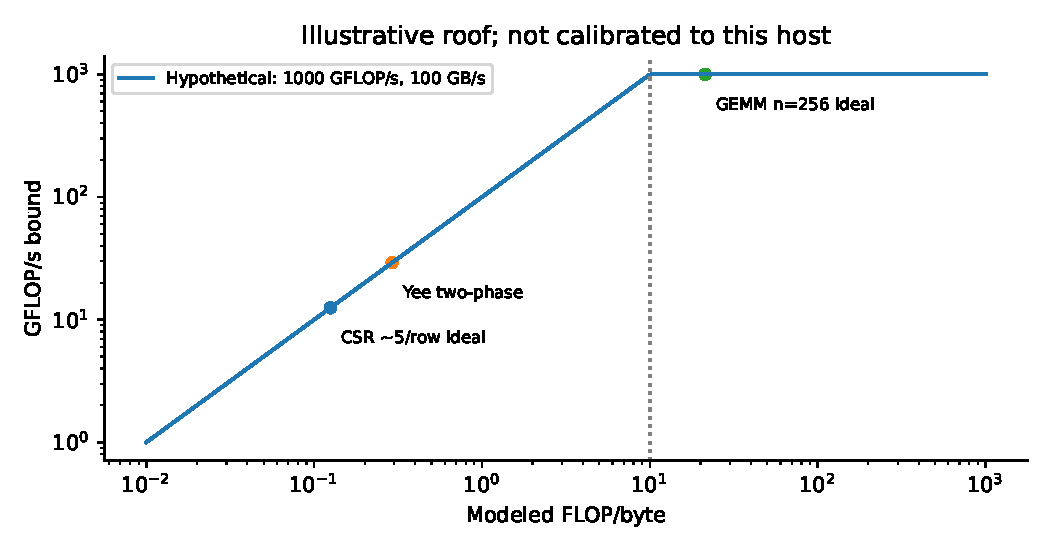
\includegraphics[width=.84\textwidth]{Vol0_Linear_Algebra_HPC/figures/roofline_model.pdf}}{}
\caption{假设硬件的 Roofline 示意；屋顶与字节模型均非 DRAM 计数器实测。}
\end{figure}
标定时需分别测持续带宽、对应精度计算吞吐及真实数据流量；不同缓存层级可建立不同屋顶。小数组驻留缓存时，DRAM 流量模型不适用。
\costnote{带宽受限核优先减少流量、改善复用与布局；计算受限核优先提升向量化和指令效率。GFLOP/s 用于定位资源利用，固定误差下的总时间用于评价计算收益。}
\coderef{roofline/kernels.py}
\aiexercise{对 32 位与 64 位索引 CSR 分别推导理想和逐非零读取 $x$ 的字节模型，计算强度，并说明写分配遗漏在哪里。}{给定 GEMM、SpMV 的实际计时和数组大小，判断能否把它们放到同一 DRAM Roofline；列出还缺的测量。}
\studyroute{略去硬件计数器校准与经验多层 Roofline 工具实现。参考 \cite{roofline,cuda}。}{arithmetic intensity; operational intensity; ridge point; sustained bandwidth; hierarchical Roofline}

\chapter{离散方法的计算与访存指纹}\label{v0ch:23}
\begin{chaptersummary}
Roofline 分析需要具体算子的工作量与数据流量。本章据此比较差分、有限体积、有限元、DG、FR 与 LBM，联系自由度、局部性、阶数和几何对复用的影响。这些计算与访存特征构成方法的性能指纹，下一章的 Yee 更新和后续综合实验将给出可运行的实例。
\end{chaptersummary}
\learninggoals{构造各方法的工作量和访问模型；区分装配与矩阵自由；比较体项、面项及迁移碰撞。}
\paragraph{核心问题}空间离散如何决定机器实际读取和计算什么？

\section{差分与有限体积}
三维七点 Laplacian 可按
\[
 (\bm L u)_{ijk}
 =h^{-2}(u_{i+1,j,k}+u_{i-1,j,k}+u_{i,j+1,k}
 +u_{i,j-1,k}+u_{i,j,k+1}+u_{i,j,k-1}-6u_{ijk})
\]
计算。按五次邻值求和、一次乘 6、一次相减和一次缩放共 8 FLOPs。每点七读一写的语义流量为 64 bytes；理想空间复用下可接近每点一读一写的 16 bytes，均未计写分配。缓存分块和时间分块分别改善空间与跨步复用；边界和依赖限制其规模。
有限体积包含梯度重构、限制器、面 Riemann 通量和残量累加。非结构面访问可能产生 gather/scatter；每面只算一次可减少重复计算，但并行累加需着色、原子或面缓冲。每单元独立遍历则避免冲突而增加重复通量。两者应在同一精度与守恒条件下比较。
\section{有限元、DG 与 FR}
低阶装配 FEM 的主核可为稀疏矩阵乘；装配过程还涉及求积、几何和稀疏累加。矩阵自由重新执行单元算子，以计算换取条目与索引流量。
三维张量单元每方向 $n=p+1$ 点，直接稠密体算子可达 $O(n^6)$，和因子分解将三个方向导数降为 $O(n^4)$：
\[
 (\partial_\xi u)_{ijk}=\sum_{\ell=0}^{p}D_{i\ell}u_{\ell jk}.
\]
三个方向各执行 $n^3$ 个长度 $n$ 点积，计 $3n^3(2n-1)$ FLOPs。若一次读输入、写三组输出，最低场数据流量约 $32n^3$ bytes，另计导数矩阵、几何和材料。实际批量、寄存器压力及面数据改变复用。
DG 的体项、面通量与提升操作可分别建模；FR 由点值导数与界面通量差修正组成，两者在张量网格上均可利用局部矩阵乘。它们的算子关系由校正函数、求积与节点共同确定，稳定性则进一步通过相应能量或谱估计检验。
\conceptbridge{高阶每单元做更多运算，为何仍可能更快？}{增加阶数可能提高数据复用并以较少单元达到目标误差；同时自由度、面成本和显式稳定步长也会改变。只有把空间误差、时间误差和总步数同时计入，才能评价收益。}{局部高阶运算 $\longrightarrow$ 复用与误差变化 $\longrightarrow$ 总成本比较。}
\section{LBM 的迁移与碰撞}
每格点保存 $Q$ 个分布分量，BGK 碰撞为
\[
 f_q^*=f_q-\tau^{-1}(f_q-f_q^{\rm eq}),\qquad
 f_q(\bm x+\bm c_q\Delta t,t+\Delta t)=f_q^*(\bm x,t).
\]
D2Q9、D3Q19、D3Q27 分别有 9、19、27 个分量。双缓冲迁移最低读写约 $2Q$ 个标量；双精度 D2Q9 为 144 bytes/格点，尚未计碰撞临时量和边界。
SoA 将同一方向的连续格点排在一起，AoS 将同格点分量排在一起；适用性取决于 SIMD/SIMT 映射及碰撞实现。push 将后碰撞值写到邻点，pull 从邻点读取；周期单射迁移可避免冲突，复杂边界需另行处理。
\section{统一比较表}
\begin{center}\small
\begin{tabularx}{\textwidth}{lXX}
\toprule 方法&主要复用与访问&常见限制\\\midrule
FDM&规则邻点、跨点复用&带宽、边界、时间步\\
FVM&面几何、重构与通量&非规则访问、分支、累加\\
FEM&局部求积或稀疏乘&装配与应用路径不同\\
DG&体张量与面数据&寄存器、提升、稳定步长\\
FR&点导数与通量修正&节点和校正函数、面通信\\
LBM&方向分量迁移与碰撞&布局、存储、复杂边界\\
FDTD&交错旋度 stencil&两相依赖、带宽、色散\\\bottomrule
\end{tabularx}
\end{center}
\costnote{表中按访问特征定位瓶颈。比较方法时，固定物理问题、误差、精度、硬件和并行规模；分析 NumPy 实现时，再将临时数组流量计入理想融合核模型。}
\coderef{roofline/kernels.py; dg_fr/transport.py; lbm/stream_collision.py}
\aiexercise{为七点 Laplacian、三维张量导数和 D2Q9 迁移分别列运算与读写表，明确哪些读可由缓存复用。}{用相同周期正弦输运比较一阶上风 FVM 与高阶 DG 的空间误差、步数和总时间；不要把 LBM 的流体模型与任意标量方程直接等同。}
\studyroute{略去一般曲边和因子分解及 FR 能量稳定性证明。参考 \cite{hesthaven,vcjh,frdisp,roofline}。}{sum factorization; matrix-free FEM; DG volume surface; FR correction; LBM SoA AoS}

\chapter{Yee-FDTD：离散结构与性能}\label{v0ch:24}
\begin{chaptersummary}
第二卷建立了 Maxwell 演化与约束的相容离散。本章沿 Yee 网格的自由度、交错时间和旋度结构，将拓扑恒等式落实为数组更新，再分析工作量与流量。由此，离散复形、相位关系和两相数据依赖成为性能优化的明确约束。
\end{chaptersummary}
\learninggoals{写出 Yee 更新与离散约束；区分关联矩阵和材料 Hodge；计算三种流量口径并检验色散与能量。}
\paragraph{核心问题}怎样在保持 Maxwell 结构的同时识别 Yee 实现的性能瓶颈？

\section{自由度、材料与网格}
取静止、无色散各向同性介质：
\[
 \varepsilon\partial_t\bm E=\nabla\times\bm H-\bm j,\qquad
 \partial_t\bm B=-\nabla\times\bm E,\qquad \bm B=\mu\bm H.
\]
$\varepsilon,\mu$ 显式保留在材料与波速关系中。立方格上 $E_x$ 位于 $(i+\tfrac12,j,k)$，$E_y,E_z$ 循环换位；$B_x$ 位于 $(i,j+\tfrac12,k+\tfrac12)$，其余同理。$E$ 在整数时间，$B$ 在半整数时间。

\begin{figure}[H]\centering
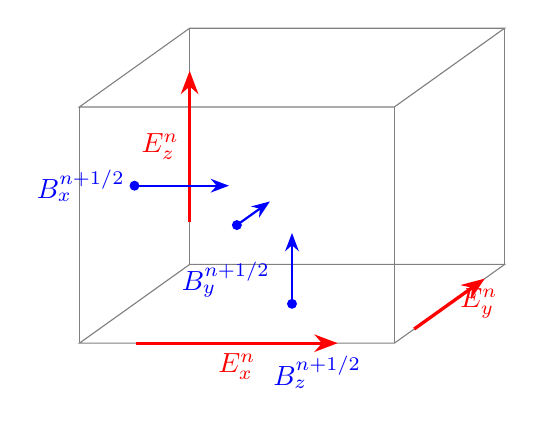
\begin{tikzpicture}[x={(4cm,0cm)},y={(1.4cm,1cm)},z={(0cm,3cm)},>=Stealth]
\foreach \z in {0,1}{\draw[gray] (0,0,\z)--(1,0,\z)--(1,1,\z)--(0,1,\z)--cycle;}
\foreach \x in {0,1}{\foreach \y in {0,1}{\draw[gray] (\x,\y,0)--(\x,\y,1);}}
\draw[very thick,red,->](.18,0,0)--(.82,0,0) node[midway,below]{$E_x^n$};
\draw[very thick,red,->](1,.18,0)--(1,.82,0) node[midway,right]{$E_y^n$};
\draw[very thick,red,->](0,1,.18)--(0,1,.82) node[midway,left]{$E_z^n$};
\fill[blue] (0,.5,.5) circle(1.8pt);
\draw[blue,thick,->](0,.5,.5)--(.3,.5,.5);
\node[blue,anchor=east] at (0,.5,.5) {$B_x^{n+1/2}$};
\fill[blue] (.5,0,.5) circle(1.8pt);
\draw[blue,thick,->](.5,0,.5)--(.5,.3,.5);
\node[blue,anchor=north] at (.5,-.1,.42) {$B_y^{n+1/2}$};
\fill[blue] (.5,.5,0) circle(1.8pt);
\draw[blue,thick,->](.5,.5,0)--(.5,.5,.3);
\node[blue,anchor=north] at (.58,.5,-.18) {$B_z^{n+1/2}$};
\end{tikzpicture}
\caption{单个立方胞元的代表性边电场与面磁场位置。箭头标记分量方向，不表示全部边面自由度。}
\end{figure}

点值分量可看作均匀网格上的采样；积分自由度则为边环量 $e_\ell=\int_\ell E$ 与面通量 $b_f=\int_f B$。边长、面积及材料因子把两种记法联系起来，不能将点值数组直接称为无量纲关联矩阵。
\section{拓扑与矩阵自由更新}
边界关联矩阵为 $G,C,D$，满足 $CG=0,DC=0$。在相容原始/对偶网格和边界配对下，可写
\[
 \dot{\bm b}=-C\bm e,\qquad
 M_\varepsilon\dot{\bm e}=C^TM_{\mu^{-1}}\bm b-\bm j_h .
\]
$C$ 编码取向，$M_\varepsilon,M_{\mu^{-1}}$ 编码度量和材料；均匀正交 Yee 网格可采用对角材料作用。于是 $\partial_t(D\bm b)=0$。采用对偶散度 $D_e=-G^T$ 的取向约定，离散电荷为 $\bm q=D_eM_\varepsilon\bm e$，连续性更新需满足 $\dot{\bm q}=-D_e\bm j_h$；边界通量也必须相容。
定义前向差分 $\delta_\alpha^+$ 和后向差分 $\delta_\alpha^-$，周期均匀网格上
\[
 B_x^{n+1/2}=B_x^{n-1/2}
 -\Delta t(\delta_y^+E_z^n-\delta_z^+E_y^n),
\]
\[
 E_x^{n+1}=E_x^n+\frac{\Delta t}{\varepsilon}
 [\delta_y^-H_z^{n+1/2}-\delta_z^-H_y^{n+1/2}-j_x^{n+1/2}],
\]
其余循环换位。它是块稀疏算子作用，但无需装配 CSR；显式矩阵表示则便于小规模谱分析、隐式积分和不同离散算子的核对。基本执行顺序为
\begin{quote}\ttfamily\small
for each time step:\\
\quad exchange required E halos\\
\quad B\_half = B\_half - dt * curl\_forward(E)\\
\quad exchange required B\_half halos\\
\quad E = E + dt * curl\_backward(B\_half)
\end{quote}
\conceptbridge{为什么相同的旋度公式不能任意改成就地更新？}{两个旋度必须使用各自一致的时间层和空间取向。半步磁场依赖旧电场，整步电场依赖新磁场；覆盖尚未读取的数据会改变离散算子，破坏稳定性、色散和离散约束。}{交错自由度 $\longrightarrow$ 两相依赖图 $\longrightarrow$ 允许的融合与同步。}
\section{可审核的工作量与流量}
无源、真空、常系数且预先计算倒网格距时，每个分量更新：两次差、两次尺度乘、一次差、一次 $\Delta t$ 乘和一次加减，共 7 FLOPs；六分量整步为 42 FLOPs/胞元。FMA 仍按两 FLOPs 计。
这一计数对应先计算各向差分再乘时间步的实现。各向同性等距网格可预合并 $\Delta t/h$，每分量变为三次相减、一次尺度乘和一次更新，共 5 FLOPs，整步 30 FLOPs；附带 CUDA 与 MPI 程序采用此形式。报告吞吐时按各自实现计数，不能给融合核沿用 42 FLOPs。
双精度不含材料与源项时：
\[
\begin{array}{l|r|r}
\text{模型}&\text{bytes/胞元整步}&I\ (\text{FLOP/byte})\\\hline
\text{每分量四邻读+自身读+写}&288&42/288\\
\text{每相输入各读一次、输出写一次}&144&42/144\\
\text{整步六数组全驻留的读写下界}&96&42/96
\end{array}
\]
三个数字分别对应指定复用假设下的流量模型。实际 DRAM 流量还包括缓存行为、写分配、临时数组、边界和系数访问；两相大数组实现需据工作集大小判断整步数据能否驻留。
SoA 的六个连续数组适合让相邻线程访问相邻空间点。GPU 核可按 $B/E$ 分两次启动，必要时再拆分分量；寄存器、启动开销和全局同步共同决定取舍。shared memory 只有在减少实际重复搬运且不压低并行度时才有收益。
\section{稳定性、色散与验收}
真空波速 $c=(\varepsilon\mu)^{-1/2}$，均匀三维网格的条件为
\[
 c^2\Delta t^2(h_x^{-2}+h_y^{-2}+h_z^{-2})\le1.
\]
周期 Fourier 模满足
\[
 \frac{\sin^2(\omega_h\Delta t/2)}{c^2\Delta t^2}
 =\sum_\alpha\frac{\sin^2(k_\alpha h_\alpha/2)}{h_\alpha^2}.
\]
CFL 控制数值增长，色散关系刻画相位传播。评估固定距离的传播误差时，应同时记录方向、分辨率和总步数。
对周期真空归一化系统，一个精确算术守恒量是
\[
 {\cal H}^n=\frac12\norm{E^n}^2+
 \frac12\langle B^{n-1/2},B^{n+1/2}\rangle
\]
（乘相应体积权重）。它是交错修正能量，不等同于把不同时刻的平方直接相加；稳定步长下其与物理能量的关系需要明确。
\costnote{端到端实验记录初值相位、物理终止时间、误差、$\diverg_h B$、电荷残量、修正能量与推进时间。约束保持检查应同时包含非平凡随机场的离散旋度--散度测试，而不只测试单一横波。周期无耗散模式的放大因子在稳定区间内为单位模；边界、材料损耗与滤波可能引入额外耗散，需分别记录。}
\coderef{fdtd/yee.py}
\aiexercise{由本章分量位置推导 $B_x$ 和 $E_x$ 的邻点索引，逐项验证 $D C=0$；再解释面积和边长进入何处。}{从 Yee Fourier 更新推导离散色散及 CFL，比较修正交错能量与不同时刻平方和的变化。}
\crossref{第二卷讨论几何与约束来源；这里的材料质量矩阵、离散流量和时间层为第 25、28、29 章提供实现接口。}
\studyroute{略去 PML、色散材料、曲线网格 Hodge 和 PEC 边界细节。参考 \cite{yee,cuda}。}{Yee staggered grid; incidence matrix; discrete Hodge; numerical dispersion; modified energy}

\chapter{时间推进与总求解成本}\label{v0ch:25}
\begin{chaptersummary}
空间算子的吞吐给出单次调用成本，时间推进则决定调用次数与隐式求解工作。本章在统一成本框架中比较 RK、交错积分、ADER、CERK、LTS 和 IMEX，联系稳定性、相位精度与结构保持。给定目标误差和终止时间后，步长、阶段数、求解与通信才能共同确定总成本。
\end{chaptersummary}
\learninggoals{连接半离散谱与稳定域；区分保辛与能量守恒；解释高阶、局部步进与刚性分拆的成本。}
\paragraph{核心问题}一次空间算子很快，为什么完整模拟仍可能很慢？

\section{线法与稳定域}
空间离散得到 $M\dot{\bm u}=\bm R(\bm u)$；显式 RK 每阶段求 $M^{-1}\bm R$，局部或对角质量矩阵使其便宜。对 $\dot y=\lambda y$，一步为 $y^{n+1}=R(z)y^n$，$z=\Delta t\lambda$，绝对稳定要求 $|R(z)|\le1$。经典 RK4 的
$R(z)=1+z+z^2/2+z^3/6+z^4/24$。半离散算子的谱、非正规性及能量估计共同影响可用步长。
纯虚 $\lambda$ 下，前向 Euler 的 $|1+\mathrm i\omega\Delta t|>1$ 导致模态增长。这说明时间积分器的稳定域也是完整能量分析的一部分。
\section{交错、保辛与相位}
Yee/leapfrog 对适当分裂系统交错更新，具有条件稳定性。Störmer--Verlet 对可分 Hamilton 系统是二阶保辛方法。隐式中点
\[
 \frac{\bm u^{n+1}-\bm u^n}{\Delta t}
 =A\frac{\bm u^{n+1}+\bm u^n}{2}
\]
在 $A^TQ+QA=0$、$Q$ 固定 SPD 时精确保持离散二次能量；它对一般 Hamilton 系统保辛，但一般保辛不等于精确保持原 Hamilton 量。
对 $\lambda=\mathrm i\omega$，中点的相位频率为
$\omega_h=2\arctan(\omega\Delta t/2)/\Delta t$。模长稳定仍可累积相位误差；每步线性解不精确时，守恒性质也会受到影响。
\section{ADER、CERK 与 LTS}
ADER 通过单元局部时空预测构造高阶时间表示，再以界面时空通量校正；预测计算可提高局部复用，但代价、稳定性和阶数依具体实现而定。
CERK 指连续显式 Runge--Kutta：除阶段值外构造步内近似
\[
 \bm u(t_n+\theta\Delta t)
 \approx\bm u_n+\Delta t\sum_i b_i(\theta)\bm k_i,\quad0\le\theta\le1.
\]
步内精度由连续扩展的阶条件决定，终点精度则由 RK 更新的阶条件决定；两者在耦合与输出时分别检查。
LTS 将不同尺寸或局部波速的单元分层步进。相邻单元必须共享同一个时间积分通量，细步累积与粗步校正一致，才可保持守恒。插值、通量寄存器、调度和负载不均是额外成本。
\section{IMEX 与刚性源项}
分拆 $\dot{\bm u}=F(\bm u)+G(\bm u)$，显式处理传播，隐式处理刚性源项。加性 RK 的阶段为
\[
 U_i=\bm u^n+\Delta t\sum_{j<i}\widetilde a_{ij}F(U_j)
                  +\Delta t\sum_{j\le i}a_{ij}G(U_j),
\]
终点分别使用显隐权重。完整阶数与稳定性取决于成对 tableau 及耦合条件。
导电 Maxwell 中可令 $G_E=-\sigma E/\varepsilon$。一阶分拆示例为
\[
 E^{n+1}=\frac{E^n+\Delta t\,(\curl H)^n/\varepsilon}
 {1+\Delta t\,\sigma/\varepsilon}.
\]
它说明局部刚性阻尼可廉价隐式处理；若传播使用前向 Euler，$\sigma=0$ 时仍不适合纯波传播。实际选择应使用与双曲显式部分稳定域相容的 IMEX 对。全局扩散或耦合源项的隐式阶段可能重新引入大规模线性求解。
\conceptbridge{高阶或隐式方法为何不自动减少总成本？}{高阶改变每步阶段数和误差常数，隐式改变稳定限制却引入求解成本；局部时间步又改变调度与通信。必须在相同误差约束下同时确定可用步长、步数和每步执行图。}{稳定与精度要求 $\longrightarrow$ 可用时间步 $\longrightarrow$ 阶段、求解和通信总成本。}
\section{最小比较}
对周期正弦输运比较 RK4、二阶方法和交错波动更新；对 $\dot y=\mathrm i\omega y-\sigma y$ 比较显式与 IMEX 的稳定域及相位。测试目标是给定终止时间的误差，而非只画 $|R|$。
\costnote{$T_{\rm total}=T_{\rm setup}+N_tT_{\rm step}+T_{\rm output}$，其中 $T_{\rm step}$ 包含全部阶段、隐式求解与通信。ADER 和 LTS 以额外局部工作换取减少全局更新的机会；CERK 提供时间对齐状态，接口通量与组合稳定域则分别控制守恒和稳定性。}
\aiexercise{从中点放大因子推导相位频率，量化传播一百周期后的相位误差，并与 RK4 比较。}{对两个相邻不同步长单元写出共享通量积分和细步累积，指出只插值边界值为何不足以保证守恒。}
\studyroute{略去 ADER 预测器构造、CERK 阶条件和高阶 IMEX tableau 推导。接口见第二卷时间推进章及 \cite{hesthaven,ader,cerk,imex}。}{method of lines; symplectic integrator; ADER; continuous explicit Runge Kutta; conservative LTS; IMEX additive RK}

\chapter{内存层级与算子实现}\label{v0ch:26}
\begin{chaptersummary}
算子的理想流量给出了复用目标，实际实现还需确定数据经过哪些存储层。本章将寄存器、缓存和 DRAM 联系到布局、分块、融合与 SIMD，逐项分析临时量、依赖和访问路径。有效优化由此落实为减少关键层级的数据移动，并在同一误差与计时口径下检验收益。
\end{chaptersummary}
\learninggoals{分析步长与缓存复用；解释融合、分块、SIMD 和矩阵自由的取舍；设计公平计时。}
\paragraph{核心问题}理论上只需读一次的数据，程序为什么会反复搬运？

\section{层级、局部性与布局}
寄存器靠近执行单元，L1/L2/L3 缓存逐级扩大容量，DRAM 提供主要容量。具体共享方式依架构而异。连续访问有利于缓存行利用和硬件预取，跨大步长或随机 gather 可能浪费事务；工作集尺寸决定哪些复用能真正保留。
C 顺序三维数组最后一个索引连续；循环与线程映射宜使连续维成为内层。多分量 SoA 常利于跨点向量化，AoS 可能利于单点全部分量复用，AoSoA 则在小块内折中。应以实际核的数据使用方式判断。
\section{融合与分块}
表达式 $w=a u+b v$ 若先形成两个临时数组再相加，会增加写回和读取；融合可直接读 $u,v$ 写 $w$。但融合增加寄存器活跃变量，过度融合可能溢出至内存。
空间分块将 stencil 相邻平面留在缓存；时间分块跨多个时间步复用子域，必须保留依赖锥和扩大 halo。Yee 的两相更新或多阶段 RK 不能在缺少同步的条件下任意跨步融合。
张量 DG 可将导数矩阵留在缓存并批量处理单元；若同时保存三方向导数和通量，临时量可能超过寄存器或缓存。矩阵自由减少稀疏索引但增加重复几何计算，混合精度还需误差论证。
\conceptbridge{“零拷贝”或“矩阵自由”为何仍可能很慢？}{避免显式复制或矩阵条目只是减少某一类操作。缓存失配、隐式临时量、跨层迁移和额外算术仍可主导时间。应依据实际访问路径，而非接口名称判断数据流量。}{存储表示 $\longrightarrow$ 实际访问路径 $\longrightarrow$ 各层资源消耗。}
\section{SIMD 与最小实验}
SIMD 一条指令处理多个数据元素，要求独立迭代、合适布局、对齐及可处理的分支。编译器向量化报告、汇编或计数器比源代码外观更可靠。
对七点 stencil 比较连续内层与跨步长遍历，对 D2Q9 比较 SoA/AoS，对张量导数比较显式 Kronecker 与顺序收缩。计时前预热，保留输出以防消除，重复并报告统计值；大数组和缓存驻留小数组分开。
\costnote{分别报告分配时间与核函数时间，在统一计时范围下比较预分配和动态分配实现。NumPy 的各数组操作调用编译核，多操作之间的融合则取决于具体执行方式。}
\coderef{roofline/kernels.py; lbm/stream_collision.py; dg_fr/transport.py}
\aiexercise{逐数组列出 NumPy 七点 stencil 的临时量与生命周期，比较其字节数和第 23 章融合核下界。}{设计三个工作集分别小于 L1、L3 和大于末级缓存的实验，解释为什么同一强度点不能共用一个未经区分的带宽。}
\studyroute{略去缓存替换策略、编译器向量化与具体微架构端口分析。参考 \cite{roofline,cuda}。}{cache blocking; loop fusion; temporal blocking; SIMD; AoSoA; working set}

\chapter{CPU 与 GPU 并行吞吐}\label{v0ch:27}
\begin{chaptersummary}
内存布局决定单个执行流的效率，并行化还需要足够独立工作与资源供给。本章分别讨论 CPU 线程与 GPU SIMT，把占用率、事务合并和设备常驻连接到具体算子。核心是同时分析吞吐、依赖、启动与迁移成本，并用端到端计时验收加速。
\end{chaptersummary}
\learninggoals{解释 NUMA 与伪共享；区分 SIMD/SIMT；评估 coalescing、occupancy 和传输摊销。}
\paragraph{核心问题}更多线程或更高占用率，为什么不必然缩短时间？

\section{CPU 线程与存储归属}
多核并行将单元、行或网格块分配到线程；OpenMP 循环需要无冲突写入或显式同步。线程绑定与 first touch 决定 NUMA 页面归属，跨插槽访问会改变带宽和延迟。不同线程写同一缓存行的不同变量仍会产生伪共享，可用分块和适当填充分离热点。单核 SIMD 与多核线程是可组合层次。
混合核心处理器的线程性能、绑核策略和电源状态会影响短时实验。因此本卷记录 CPU 型号、可用逻辑处理器与 BLAS 线程配置；持续全核吞吐另由对应负载标定。
\section{GPU 的执行资源}
CUDA 将线程组成 block，block 调度到 SM，warp 以 SIMT 执行。\cite{cuda}
连续线程访问连续元素有利于合并全局内存事务；分支分歧、非规则 gather 和不足并行度会降低利用。寄存器和 shared memory 限制同时驻留的 block/warp，occupancy 是资源驻留比例，不是性能本身。提高 occupancy 若牺牲数据复用或增加 spill，可能无益。
SpMV 的短行与长行负载不同；DG 单元可批量映射为小矩阵核；Yee 与 LBM 宜先设计空间连续索引，再讨论共享缓存。kernel 启动具有固定开销，小问题可能由启动主导。
\section{迁移、异步与设备常驻}
\[
 T_{\rm accelerator}=T_{\rm H2D}+T_{\rm kernels}
 +T_{\rm D2H}+T_{\rm synchronization}.
\]
长时间推进应尽量保留场、几何和预条件数据在设备上。异步拷贝与计算重叠需要支持条件、合适流和缓冲管理；异步调用返回时间不等于核完成时间。使用设备事件或显式同步计时，分别报告首次启动、稳态核和包含传输的总时间。
统一内存提供共享地址与按需迁移机制，但不消除主机与设备之间的数据移动；缺页、迁移粒度及驻留位置仍影响成本。显式预取和适当的数据归属可改善某些访问模式，需与显式传输实测比较。
\conceptbridge{为什么用 CPU 时钟测一次异步调用会得到虚假的巨大加速？}{主机调用常只把工作入队，实际计算稍后在设备执行。结束计时前必须等待对应工作完成；传输和初始化是否计入也需明确。}{主机提交 $\longrightarrow$ 设备执行 $\longrightarrow$ 完成同步与有效计时。}
\section{可复现实验接口}
附带 CUDA 程序比较单分量 AoS/SoA 访问，执行两相周期 Yee 更新，并在主机复核结果。程序分别记录编译、设备可用性与数值验证状态；计时在设备执行后生成。完整实验还应记录型号、驱动、精度、block 配置、寄存器、设备带宽和传输范围。
\costnote{GPU 优势取决于工作规模与驻留时间；稀疏三角依赖、全局归约或小规模核可能限制加速。CPU 优化也需避免 BLAS 线程与外层线程过度订阅。}
\coderef{gpu/yee_layout.cu}
\aiexercise{为 SoA 与 AoS 的 $E_x$ 更新列出一个 warp 中的地址序列，估计缓存行或事务利用，再指出哪些量必须用 profiler 验证。}{给出包含传输、预热、重复执行与同步的计时方案，并推导需要多少时间步才能摊销一次设备迁移。}
\studyroute{略去特定 GPU 的指令流水与自动调优。参考 \cite{cuda}。}{OpenMP; NUMA first touch; false sharing; SIMT; coalescing; occupancy; device residency}

\chapter{分布式计算与通信成本}\label{v0ch:28}
\begin{chaptersummary}
单机计算加速后，halo 交换、全局点积和粗层通信逐渐进入关键路径。本章在计算与内存 Roofline 之外引入消息延迟和数据量，解释强弱扩展、通信进度与重叠。算子依赖决定哪些通信可被隐藏，实际计时则检验这种重叠能否兑现。
\end{chaptersummary}
\learninggoals{建立 alpha-beta 模型；区分 halo 与 allreduce；解释重叠、流水化及粗层瓶颈。}
\paragraph{核心问题}局部计算已经很快，为什么增加进程仍会停止加速？

\section{通信成本与扩展}
一次通信阶段可近似
\[
 T_{\rm comm}\approx n_{\rm msg}\alpha+V/B_{\rm net},
\]
其中 $\alpha$ 为有效消息启动延迟，$V$ 为指定计数口径的数据量，$B_{\rm net}$ 为有效带宽。协议、拓扑、拥塞和并发会改变参数。若计算、内存和网络完全不能重叠则成本相加；若理想重叠，可用最大值作为更乐观下界：
\[
 T\gtrsim\max(F/P_{\rm peak},Q/B_{\rm mem},T_{\rm comm}).
\]
该估算描述理想重叠下的资源下界；实际运行时间还由通信进度、资源争用与依赖链决定。
强扩展固定总规模，局部立方域边长 $\ell$ 缩小时体工作 $O(\ell^3)$、面交换 $O(\ell^2)$，表面积体积比增大。弱扩展固定每进程工作，仍受全局归约、网络与粗网格影响。
\section{halo、归约与重叠}
规则 stencil 交换相邻面；FVM/DG 交换邻接面值或迹，高阶增加面数据及本地工作。Yee 需按磁、电两相的数据依赖安排交换。Krylov 除算子 halo 外，还含点积 allreduce；CG 的短递推不消除全局同步，GMRES 正交化可能增加归约。
非阻塞模式先发接收与发送，计算不依赖 halo 的内部，再等待完成并处理边界。MPI 进度和实际重叠受实现与运行配置影响，应使用计时验证。\cite{mpi}
流水化 Krylov 尝试把归约与计算重叠；通信规避方法通过块或 s-step 减少同步，但可能增加基病态性、额外运算和残差漂移。需要同时检查数值稳定性。
\conceptbridge{通信量相同，为什么两个实现仍可能差很多？}{大量小消息受启动延迟支配，少量大消息更受带宽支配；通信是否位于关键路径、能否推进以及网络争用也不同。总字节数无法独立描述这些依赖。}{消息数量与大小 $\longrightarrow$ 进度和依赖 $\longrightarrow$ 关键路径时间。}
\section{最小 MPI 实验}
附带程序沿一个方向分割三维周期场，分别使用 \texttt{Sendrecv} 与 \texttt{Irecv/Isend+Waitall} 交换面，并核验全局 Fourier 模式的七点算子。记录包括进程数、局部大小、最大 rank 时间与误差。本机运行检验 MPI 语义，跨节点运行进一步测量网络扩展；多维分块还需六面交换与分区策略。
\costnote{AMG 粗层局部工作不断缩小，通信比例增大，可能需要进程聚合。算子、预条件、归约和 I/O 应分别计时，强扩展比较使用全局最慢 rank。}
\coderef{mpi/halo.cpp}
\aiexercise{对 $n^3$ 网格在 $p$ 个近立方子域上推导每进程体工作、六面 halo 字节与表面积体积比。}{写出非阻塞 halo 的事件图，标出可重叠内部和必须等待的边界，再设计判定实际通信进度的实验。}
\studyroute{略去网络拓扑建模、pipelined Krylov 误差分析及跨节点调优。参考 \cite{mpi,petsc}。}{alpha beta model; strong scaling; weak scaling; halo exchange; allreduce; pipelined Krylov; MPI progress}

\chapter{跨卷综合算例}\label{v0ch:29}
\begin{chaptersummary}
前面分别讨论了离散算子、代数算法和执行成本，本章通过可复现实验将三者重新连接。各案例先核验模型、误差与约束，再记录求解和数据移动的成本。以相同问题和目标误差比较总时间，可以将局部核函数分析转化为跨卷的完整计算决策。
\end{chaptersummary}
\learninggoals{建立统一实验记录；完成 Maxwell 与高阶输运案例；区分核基准、完整求解与跨模型比较。}
\paragraph{核心问题}怎样确认更快的程序仍解决了同一个问题？

\section{Krylov 与 AMG：从 Poisson 到预条件}
从第一卷的空间离散取二维 Dirichlet Poisson。先以已知解构造右端，确认直接法、CG 与预条件解的真实残差；再用解析连续解比较离散误差。记录自由度、$\nnz$、排序、因子填充、预条件构造、迭代、时间与误差。
采用代数制造右端 $\bm b=A\bm x_*$ 检查线性求解器，再以连续解析解检验 PDE 收敛阶，代码分别记录这两层误差。多右端实验复用相同因子，展示构造成本的摊销；两层 AMG 例则用于核验粗空间与修正机制。
Krylov 成本应拆成 SpMV、预条件、点积与正交化；AMG 则逐层记录平滑、限制、粗解与插值。小规模上，减少迭代未必抵消构造和 Python 调用成本；大规模上，粗层通信和全局归约又可能改变排序。教学例实测的是串行层次作用，分布式 AMG 的粗层扩展仍需独立实验。
\section{完整 Maxwell 推进}
取周期单位立方体、真空 $c=1$，右行横波
\[
 E_y(x,t)=\sin(2\pi(x-t)),\qquad B_z(x,t)=\sin(2\pi(x-t)).
\]
其他分量为零。分别在各自空间点和 $t=-\Delta t/2$ 初始化磁场，选
$\Delta t\le\nu h$、$\nu<1/\sqrt3$，最后一步统一调整以精确到达相同 $T$。比较两组网格上的 $L^2$ 误差、数值相位、步数和时间；初值不能把半时间层误当整层。
CPU 程序还从随机边场计算离散旋度并检验散度，监测完整推进中的 $\diverg_h B$ 与修正能量。无源电场散度检验对应零电荷；有源推广需相容电流和连续性更新。
\begin{figure}[htbp]\centering
\IfFileExists{Vol0_Linear_Algebra_HPC/figures/convergence.pdf}{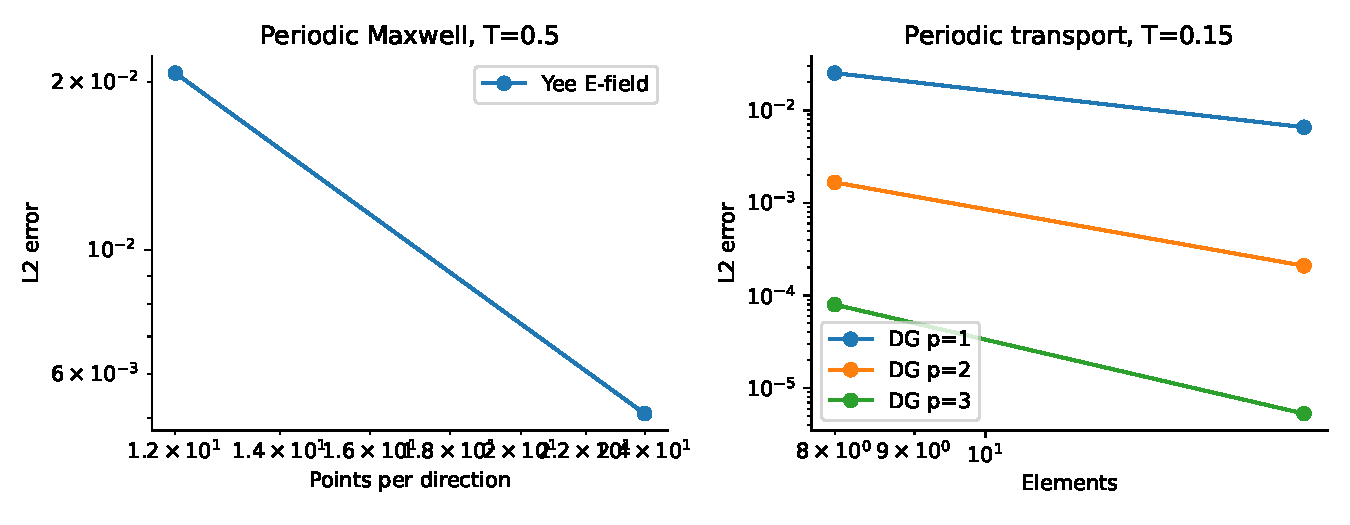
\includegraphics[width=.88\textwidth]{Vol0_Linear_Algebra_HPC/figures/convergence.pdf}}{}
\caption{本卷 CPU 程序生成的实际收敛数据：Yee 横波与周期输运。误差定义和参数见结果记录。}
\end{figure}
从 CPU 扩展到 GPU 时保留 SoA、两相顺序和初值；扩展到 MPI 时按每相交换所需分量，再做内部与边界更新。附带 CUDA 全场程序提供设备端链路，MPI 全场程序包含每相 halo 和全局约束诊断。附录与实验数据记录执行范围，跨节点与多 GPU 耦合则按同一误差和约束口径继续测量。
\section{完整高阶 DG 与 FR 接口}
对 $u_t+u_x=0$、周期 $u(x,0)=\sin(2\pi x)$，在各单元用 Legendre 模态
$u_h=\sum_{m=0}^{p}\widehat u_mP_m(\xi)$。弱形式为
\[
 \frac h2 M\dot{\widehat{\bm u}}
 =S\widehat{\bm u}-\bm\phi(1)\widehat f_R
                         +\bm\phi(-1)\widehat f_L,\quad
 M_{mm}=\frac2{2m+1},\quad S_{m\ell}=\int_{-1}^{1}P'_mP_\ell.
\]
正速度上风通量取左侧迹。体算子、面通量和对角质量逆均可直接实现。代码采用 RK4 和保守步长，比较 $p=1,2,3$ 与不同单元数的误差、自由度、步数及时间。
FR 接口实验在 $p=1$ Lobatto 两端点上，用
$g_L=(P_2-P_1)/2$、$g_R=(P_2+P_1)/2$
构造导数修正，核验它与同一精确质量及求积约定下的 nodal DG 算子等价。改变校正函数后，再比较相应提升与体积算子。三维张量导数另与稠密 Kronecker 作用对照，用于检查和因子分解。
MPI 版本按单元划分，每个 RK 阶段交换上风迹，质量逆保持单元局部。GPU 优化可将多个同阶单元批量化，复用导数矩阵并分离体项与面项；阶数增大同时提高寄存器需求和体面比。当前 GPU 可执行验证覆盖 Yee 与布局，完整 DG 的 GPU 移植作为单列扩展任务。
\conceptbridge{为什么核函数吞吐更高，完整 DG 模拟仍可能更慢？}{高阶局部运算提高算术强度，也改变时间步约束、每步阶段和误差。只有减少达到目标精度所需的总单元与总步数，局部吞吐优势才可能转化为端到端收益。}{核复用 $\longrightarrow$ 精度与稳定步长 $\longrightarrow$ 物理终止时间成本。}
\section{FDM、FVM、FEM 与 LBM 的访问对照}
同一周期输运问题还包含一阶上风 FVM，可与 DG 比较误差和总时间。FDM 七点算子、Yee、DG 张量、LBM 迁移碰撞及 CSR/GEMM 则分别展示不同访问模式。跨模型的格点更新率用于分析实现指纹，方法选型则以共同物理问题与目标误差为依据。
FEM 用装配矩阵与局部矩阵自由作用的一致性验证接口；FVM/DG 面通量检查守恒，LBM 检查周期总质量。每种实现先验收，再计时。
\subsection{规则 stencil 与交错 stencil}
七点 FDM 每次输出一个标量场；Yee 每整步更新六个交错分量并分两相读取。二者都可采用空间连续索引和 halo，但相同格点数并不表示相同自由度或相同物理问题。分别比较 8 FLOPs 的 Laplacian、42 FLOPs 的差分型 Yee 与 30 FLOPs 的融合型 Yee，并注明访问模型。
\subsection{邻接表、非规则访问与几何}
FVM 案例将非均匀周期单元重新编号，用面左右单元索引读取状态、计算通量并累加残量。验证置换前后的结果一致，且体积加权残量和为零。该例隔离编号与 gather/scatter；一般非结构网格还需面法向、面积、重构邻域和图分区。MPI 交换应由跨分区面确定，而不是假定每个单元都有固定数组邻点。
\subsection{局部矩阵与人口分布布局}
一维 P1 FEM 比较 CSR 作用与逐单元差分累加，检查同一边界消元后的输出。LBM 则分别计时迁移、碰撞和完整步：迁移布局实验验证 push/pull 及 AoS/SoA 输出相同，完整周期 BGK 实验核验总质量。GPU occupancy 还受碰撞活跃变量与边界分支影响，单个 CPU 布局测试无法预测该量。
\paragraph{八组案例的对应关系}
FDM--Yee 的 stencil 对照、FVM 邻接、DG/FR 体面结构、LBM 迁移碰撞、Krylov、AMG、完整 Maxwell 和完整高阶 DG 分别覆盖本卷的八个性能接口。各自的数值验收与执行范围在代码和附录中记录。
\section{统一验收与选择}
\begin{center}\small
\begin{tabularx}{\textwidth}{lX}
\toprule 维度&应记录内容\\\midrule
物理与离散&方程、边界、初值、$T$、网格、阶数、自由度\\
数值准确性&空间/时间误差、相位、真实残差、守恒与约束\\
算法工作&时间步、阶段、迭代、预条件与层次复杂度\\
资源&数组/因子内存、模型 FLOPs、模型流量、消息与归约\\
执行范围&构造、推进、传输、通信、验证及输出是否计入\\\bottomrule
\end{tabularx}
\end{center}
\costnote{固定自由度比较用于分析实现，固定误差比较用于选择方案；两种实验都应报告。附带小规模 CPU 测试验证流程，大规模优化还需真实工作集、并行规模与硬件计数器。}
\coderef{run_all.py; run_accelerators.py; fdtd/yee.py; dg_fr/transport.py}
\aiexercise{运行本卷实验，从 JSON 生成误差--时间与误差--自由度图。先检查每条曲线的物理问题、终止时间和误差范数是否一致。}{选择一个误差阈值，为 Yee 或 DG 设计网格、阶数和时间步联合搜索；将构造、通信与输出纳入端到端预算。}
\studyroute{跨节点硬件基准与工程级复杂边界应用留待进一步实验，复现命令和计时约定见实验指南。参考 \cite{yee,hesthaven,roofline}。}{verification versus validation; manufactured solution; error versus cost; constraint preservation; time to solution}

\appendix
\chapter{实验复现与记录口径}
在仓库根目录执行 \texttt{make vol0-examples} 生成 CPU 实验、图和 JSON 记录，再执行 \texttt{make vol0} 编译本卷。依赖为 Python、NumPy、SciPy、Matplotlib 和 XeLaTeX。实验默认单线程 BLAS，避免将线程配置差异混入算法比较。
\par
\path{results/measurements.json} 记录环境、参数、时间、残差和误差。\path{results/validation.json} 保存不依赖计时的断言。字节数采用指定工作量模型，\texttt{dram\_bytes\_measured} 保持为空，表示没有使用硬件计数器；以该模型计算的有效带宽不能解释为 DRAM 带宽实测。
\par
GPU 与 MPI 源程序分别位于示例目录的 \texttt{gpu/} 和 \texttt{mpi/}。实验按编译、设备数值验证与跨节点性能三个层次记录，执行命令和计时约定见 \path{docs/experiments.md}。附图由代码生成，计时对应记录中的实现、工作负载与硬件配置。
\section{误差与成本的共同记录}
每个完整演化实验应记录：方程和边界、初值、物理终止时间、网格与阶数、自由度、时间步和步数、精度、误差范数、约束量、预处理时间、推进时间以及硬件与线程配置。固定网格的核函数吞吐与固定误差的总求解时间分别报告。
\section{结果的可迁移性}
改变处理器、电源模式、线程数、编译器或库版本后，应重新标定。缓存驻留数组采用对应缓存层级的屋顶；含 Python 临时数组的实现将中间读写纳入流量模型。跨节点实验进一步记录网络、进程绑定、消息大小和归约策略。
\InputIfFileExists{Vol0_Linear_Algebra_HPC/results/summary.tex}{}{}

\backmatter
\begin{thebibliography}{99}
\addcontentsline{toc}{chapter}{参考文献}
\bibitem{golub} Golub G H, Van Loan C F. \emph{Matrix Computations}. 4th ed. Johns Hopkins University Press, 2013.
\bibitem{trefethen} Trefethen L N, Bau D. \emph{Numerical Linear Algebra}. SIAM, 1997.
\bibitem{saad} Saad Y. \emph{Iterative Methods for Sparse Linear Systems}. 2nd ed. SIAM, 2003. \url{https://www-users.cse.umn.edu/~saad/IterMethBook_2ndEd.pdf}.
\bibitem{templates} Barrett R, et al. \emph{Templates for the Solution of Linear Systems}. SIAM, 1994. \url{https://www.netlib.org/templates/templates.pdf}.
\bibitem{briggs} Briggs W L, Henson V E, McCormick S F. \emph{A Multigrid Tutorial}. 2nd ed. SIAM, 2000.
\bibitem{trottenberg} Trottenberg U, Oosterlee C W, Schüller A. \emph{Multigrid}. Academic Press, 2001.
\bibitem{architecture} Hennessy J L, Patterson D A. \emph{Computer Architecture: A Quantitative Approach}. 6th ed. Morgan Kaufmann, 2017.
\bibitem{roofline} Williams S, Waterman A, Patterson D. Roofline: An Insightful Visual Performance Model for Multicore Architectures. \emph{Communications of the ACM}, 2009, 52(4):65--76. DOI:10.1145/1498765.1498785. 原始技术报告：\url{https://www2.eecs.berkeley.edu/Pubs/TechRpts/2008/EECS-2008-134.html}.
\bibitem{yee} Yee K S. Numerical solution of initial boundary value problems involving Maxwell's equations in isotropic media. \emph{IEEE Transactions on Antennas and Propagation}, 1966, 14(3):302--307. DOI:10.1109/TAP.1966.1138693.
\bibitem{hesthaven} Hesthaven J S, Warburton T. \emph{Nodal Discontinuous Galerkin Methods}. Springer, 2008.
\bibitem{bossavit} Bossavit A. \emph{Computational Electromagnetism: Variational Formulations, Complementarity, Edge Elements}. Academic Press, 1998.
\bibitem{monk} Monk P. \emph{Finite Element Methods for Maxwell's Equations}. Oxford University Press, 2003.
\bibitem{vcjh} Vincent P E, Castonguay P, Jameson A. A New Class of High-Order Energy Stable Flux Reconstruction Schemes. \emph{Journal of Scientific Computing}, 2011, 47:50--72. DOI:10.1007/s10915-010-9420-z.
\bibitem{frdisp} Vincent P E, Castonguay P, Jameson A. Insights from von Neumann analysis of high-order flux reconstruction schemes. \emph{Journal of Computational Physics}, 2011, 230:8134--8154. DOI:10.1016/j.jcp.2011.07.013.
\bibitem{ader} Dumbser M, Zanotti O, Hidalgo A, Balsara D S. ADER-WENO Finite Volume Schemes with Space-Time Adaptive Mesh Refinement. \url{https://arxiv.org/abs/1212.3585}.
\bibitem{cerk} Zennaro M. Natural continuous extensions of Runge--Kutta methods. \emph{Mathematics of Computation}, 1986, 46. 作者机构记录：\url{https://arts.units.it/handle/11368/1703220}.
\bibitem{imex} Kennedy C A, Carpenter M H. \emph{Additive Runge--Kutta Schemes for Convection--Diffusion--Reaction Equations}. NASA/TM-2001-211038, 2001. \url{https://ntrs.nasa.gov/api/citations/20010075154/downloads/20010075154.pdf}.
\bibitem{cuda} NVIDIA. \emph{CUDA Programming Guide}; \emph{CUDA C++ Best Practices Guide}. \url{https://docs.nvidia.com/cuda/cuda-programming-guide/}; \url{https://docs.nvidia.com/cuda/cuda-c-best-practices-guide/index.html}. 检索日期：2026-11-10.
\bibitem{mpi} MPI Forum. \emph{MPI: A Message-Passing Interface Standard, Version 4.1}. 2023. \url{https://www.mpi-forum.org/docs/mpi-4.1/mpi41-report.pdf}.
\bibitem{petsc} PETSc. \emph{KSP: Linear System Solvers}; \emph{KSPFGMRES}. \url{https://petsc.org/release/manual/ksp/}; \url{https://petsc.org/release/manualpages/KSP/KSPFGMRES/}. 检索日期：2026-11-10.
\bibitem{scipy} SciPy. \emph{Sparse Linear Algebra Reference}. \url{https://docs.scipy.org/doc/scipy/reference/sparse.linalg.html}. 实验版本：1.15.3；GMRES 回调与停止准则以该版本接口及实际验证为准。
\end{thebibliography}

\end{document}
